% Options for packages loaded elsewhere
\PassOptionsToPackage{unicode}{hyperref}
\PassOptionsToPackage{hyphens}{url}
%
\documentclass[
]{article}
\usepackage{amsmath,amssymb}
\usepackage{iftex}
\ifPDFTeX
  \usepackage[T1]{fontenc}
  \usepackage[utf8]{inputenc}
  \usepackage{textcomp} % provide euro and other symbols
\else % if luatex or xetex
  \usepackage{unicode-math} % this also loads fontspec
  \defaultfontfeatures{Scale=MatchLowercase}
  \defaultfontfeatures[\rmfamily]{Ligatures=TeX,Scale=1}
\fi
\usepackage{lmodern}
\ifPDFTeX\else
  % xetex/luatex font selection
\fi
% Use upquote if available, for straight quotes in verbatim environments
\IfFileExists{upquote.sty}{\usepackage{upquote}}{}
\IfFileExists{microtype.sty}{% use microtype if available
  \usepackage[]{microtype}
  \UseMicrotypeSet[protrusion]{basicmath} % disable protrusion for tt fonts
}{}
\makeatletter
\@ifundefined{KOMAClassName}{% if non-KOMA class
  \IfFileExists{parskip.sty}{%
    \usepackage{parskip}
  }{% else
    \setlength{\parindent}{0pt}
    \setlength{\parskip}{6pt plus 2pt minus 1pt}}
}{% if KOMA class
  \KOMAoptions{parskip=half}}
\makeatother
\usepackage{xcolor}
\usepackage[margin=1in]{geometry}
\usepackage{graphicx}
\makeatletter
\def\maxwidth{\ifdim\Gin@nat@width>\linewidth\linewidth\else\Gin@nat@width\fi}
\def\maxheight{\ifdim\Gin@nat@height>\textheight\textheight\else\Gin@nat@height\fi}
\makeatother
% Scale images if necessary, so that they will not overflow the page
% margins by default, and it is still possible to overwrite the defaults
% using explicit options in \includegraphics[width, height, ...]{}
\setkeys{Gin}{width=\maxwidth,height=\maxheight,keepaspectratio}
% Set default figure placement to htbp
\makeatletter
\def\fps@figure{htbp}
\makeatother
\setlength{\emergencystretch}{3em} % prevent overfull lines
\providecommand{\tightlist}{%
  \setlength{\itemsep}{0pt}\setlength{\parskip}{0pt}}
\setcounter{secnumdepth}{-\maxdimen} % remove section numbering

\newcommand{\beginsupplement}{%
        \setcounter{table}{0}
        \renewcommand{\thetable}{S\arabic{table}}%
        \setcounter{figure}{0}
        \renewcommand{\thefigure}{S\arabic{figure}}%
     }

\usepackage{lineno}
\linenumbers

\usepackage[compress, super]{natbib}

\usepackage{setspace} \doublespacing
\ifLuaTeX
  \usepackage{selnolig}  % disable illegal ligatures
\fi
\IfFileExists{bookmark.sty}{\usepackage{bookmark}}{\usepackage{hyperref}}
\IfFileExists{xurl.sty}{\usepackage{xurl}}{} % add URL line breaks if available
\urlstyle{same}
\hypersetup{
  pdftitle={Transcripts with high distal heritability mediate genetic effects on complex traits},
  hidelinks,
  pdfcreator={LaTeX via pandoc}}

\title{Transcripts with high distal heritability mediate genetic effects
on complex traits}
\author{}
\date{\vspace{-2.5em}}

\begin{document}
\maketitle

\subsection{Abstract}\label{abstract}

The transcriptome is increasingly viewed as a bridge between genetic
risk factors for complex disease and their associated pathophysiology.
Powerful insights into disease mechanism can be made by linking genetic
variants affecting gene expression (expression quantiatitive trait loci
- eQTLs) to phenotypes.

\subsection{Introduction}\label{introduction}

In the quest to understand the genetic architecture of complex traits,
gene expression is an important bridge between genotype and phenotype.
By identifying mediating transcripts, we get one step closer to a
molecular understanding of how genetic variants influence traits.
Moreover, there is evidence from genome-wide association studies (GWAS)
that regulation of gene expression accounts for the bulk of the genetic
effect on complex traits, as most trait-associated variants lie in gene
regulatory regions \cite{pmid22955828, 
pmid25363779, pmid21617055, pmid19474294, pmid24702953, 
pmid24316577, pmid27126046}. It is widely assumed that these variants
influence local transcription, and methods such as transcriptome-wide
association studies (TWAS)
\cite{pmid33020666, pmid26258848, pmid27019110, pmid26854917}, summary
data-based Mendelian randomization (SMR) \cite{pmid27019110}, and others
have capitalized on this idea to identify genes associated with multiple
disease traits \cite{pmid29567659, pmid35533209, pmid27309819, 
pmid30950127}

Despite the great promise of these methods, however, they have not been
as widely successful as it seemed they could have been, and the vast
majority of complex trait heritability remains unexplained. Although
trait-associated variants tend to lie in non-coding, regulatory regions,
they often do not have detectable effects on gene expression
\cite{pmid32912663} and tend not to co-localize with expression
quantitative trait loci (eQTLs) \cite{pmid36515579, pmid37857933}.

One possible explanation for these observations is that gene expression
is not being measured in the appropriate cell types and thus true eQTLs
influencing traits cannot be detected \cite{pmid32912663}. An
alternative explanation that has been discussed in recent years is that
effects of these variants are mediated not through local regulation of
gene expression, but through distal regulation
\cite{pmid37857933, pmid32424349, 
pmid32831138, pmid30950127}.

However, assessing the role of wide-spread distal gene regulation on
complex traits requires large, dedicated data sets that include
high-dimensional, clinically relevant phenotyping, dense genotyping in a
highly recombined population, and transcriptome-wide measurements of
gene expression in multiple tissues. Measuring gene expression in
multiple tissues is critical to adequately assess the extent to which
local gene regulation varies across multiple tissues and whether such
variablilty might account for previous failed attempts to identify
trait-relevant local eQTL. Such data sets are extremely difficult to
obtain in human populations, particularly in the large numbers of
subjects required for statistical testing. Thus, to investigate further
the role of local and distal gene regulation on complex traits, we have
generated an appropriate data set in a large population of diversity
outbred (DO) mice \cite{pmid22892839} in a population model of
diet-induced obesity and metabolic disease \cite{pmid29567659}.

The DO mice were derived from eight inbred founder mouse strains, five
classical lab strains, and three strains more recently derived from wild
mice \cite{pmid22892839}. They represent three subspecies of mouse
\textit{Mus musculus domesticus}, \textit{Mus musculus musculus}, and
\textit{Mus musculus casteneus}, and capture 90\% of the known variation
in laboratory mice {[}cite{]}. They are maintained with a breeding
scheme that ensures equal contributions from each founder across the
genome thus rendering almost the whole genome visible to genetic inquiry
\cite{pmid22892839}. We measured clinically relevant metabolic traits,
including body weight, plasma levels of insulin and glucose, and plasma
lipids in 500 DO mice. We further measured transcriptome-wide gene
expression in four tissues related to metabolic disease: adipose tissue,
pancreatic islets, liver, and skeletal muscle.

To assess the role of gene regulation in mediating variation in
metabolic traits in this population, we propose high-dimensional
mediation (HDM). In univariate approaches, such as TWAS, SMR, and other
Mendelian randomization approaches, each transcript is tested
independently for mediation of a local variant on a trait. This process
requires huge numbers of statistical tests, which is compuatationally
expensive, requires strict corrections for multiple testing, and assumes
independence of genetic variants and transcripts. Such methods are
therefore limited to detecting only the largest statistical effects and
are biased toward local gene regulation. In contrast, with
high-dimensional mediation we assessed broad relationships among the
genome, transcriptome, and phenome as a whole and identified a highly
heritable composite trait that was perfectly mediated by a composite
transcript. We show that composite transcripts were tissue-specific and
highly interpretable in terms of biological processes as well as cell
type composition. Heritability analysis of the transcripts showed that
the strongest transcriptional mediators of metabolic disease had low
local heritability and high distal heritability. Finally, we show that
the composite transcripts identified in the DO population predicted
obesity in an independent population of Collaborative Cross recombinant
inbred (CC-RIX) mice and in human subjects. In contrast, local eQTL were
unable to predict obesity in the CC-RIX mice. Together our results
suggest that both the tissue used for gene expression analysis as well
as distal gene regulation are critically important in identifying
transcriptional mediators of the genome on complex traits.

\subsection{Results}\label{results}

\subsubsection{Genetic variation contributed to wide phenotypic
variation}\label{genetic-variation-contributed-to-wide-phenotypic-variation}

Although the environment was consistent across all animals, the genetic
diversity present in this population resulted in widely varying
distributions across physiological measurements (Fig.
\ref{fig:trait_overview}). For example, body weights of adult
individuals varied from less than the average adult B6 body weight to
several times the body weight of a B6 adult in both sexes (Fig.
\ref{fig:trait_overview}A). Fasting blood glucose (FBG) also varied
considerably (Fig. \ref{fig:trait_overview}B) although few of the
animals had FBG levels that would indicate pre-diabetes ( animals, ), or
diabetes (7 animals, 1.4) according to previously developed cutoffs
(pre-diabetes: FBG \(\geq\) 250 mg/dL, diabetes: FBG \(\geq\) 300,
mg/dL) \cite{pmid17018838}. Males had higher FBG than females on average
(Fig. \ref{fig:trait_overview}C) as has been observed before suggesting
either that males were more susceptible to metabolic disease on the
high-fat diet, or that males and females may require different
thresholds for pre-diabetes and diabetes.

Body weight was strongly positively correlated with food consumption
(Fig. \ref{fig:trait_overview}D \(R^2 =\) 0.51, \(p=\)
\ensuremath{1.5\times 10^{-75}}) and fasting blood glucose (FBG) (Fig.
\ref{fig:trait_overview}E, \(R^2=\) 0.21, \(p =\)
\ensuremath{1.4\times 10^{-26}}) suggesting a link between behavioral
factors and metabolic disease. However, the heritability of this trait
and others (Fig. \ref{fig:trait_overview}F) indicates that background
genetics contribute substantially to correlates of metabolic disease in
this population.

\begin{figure}[ht!]
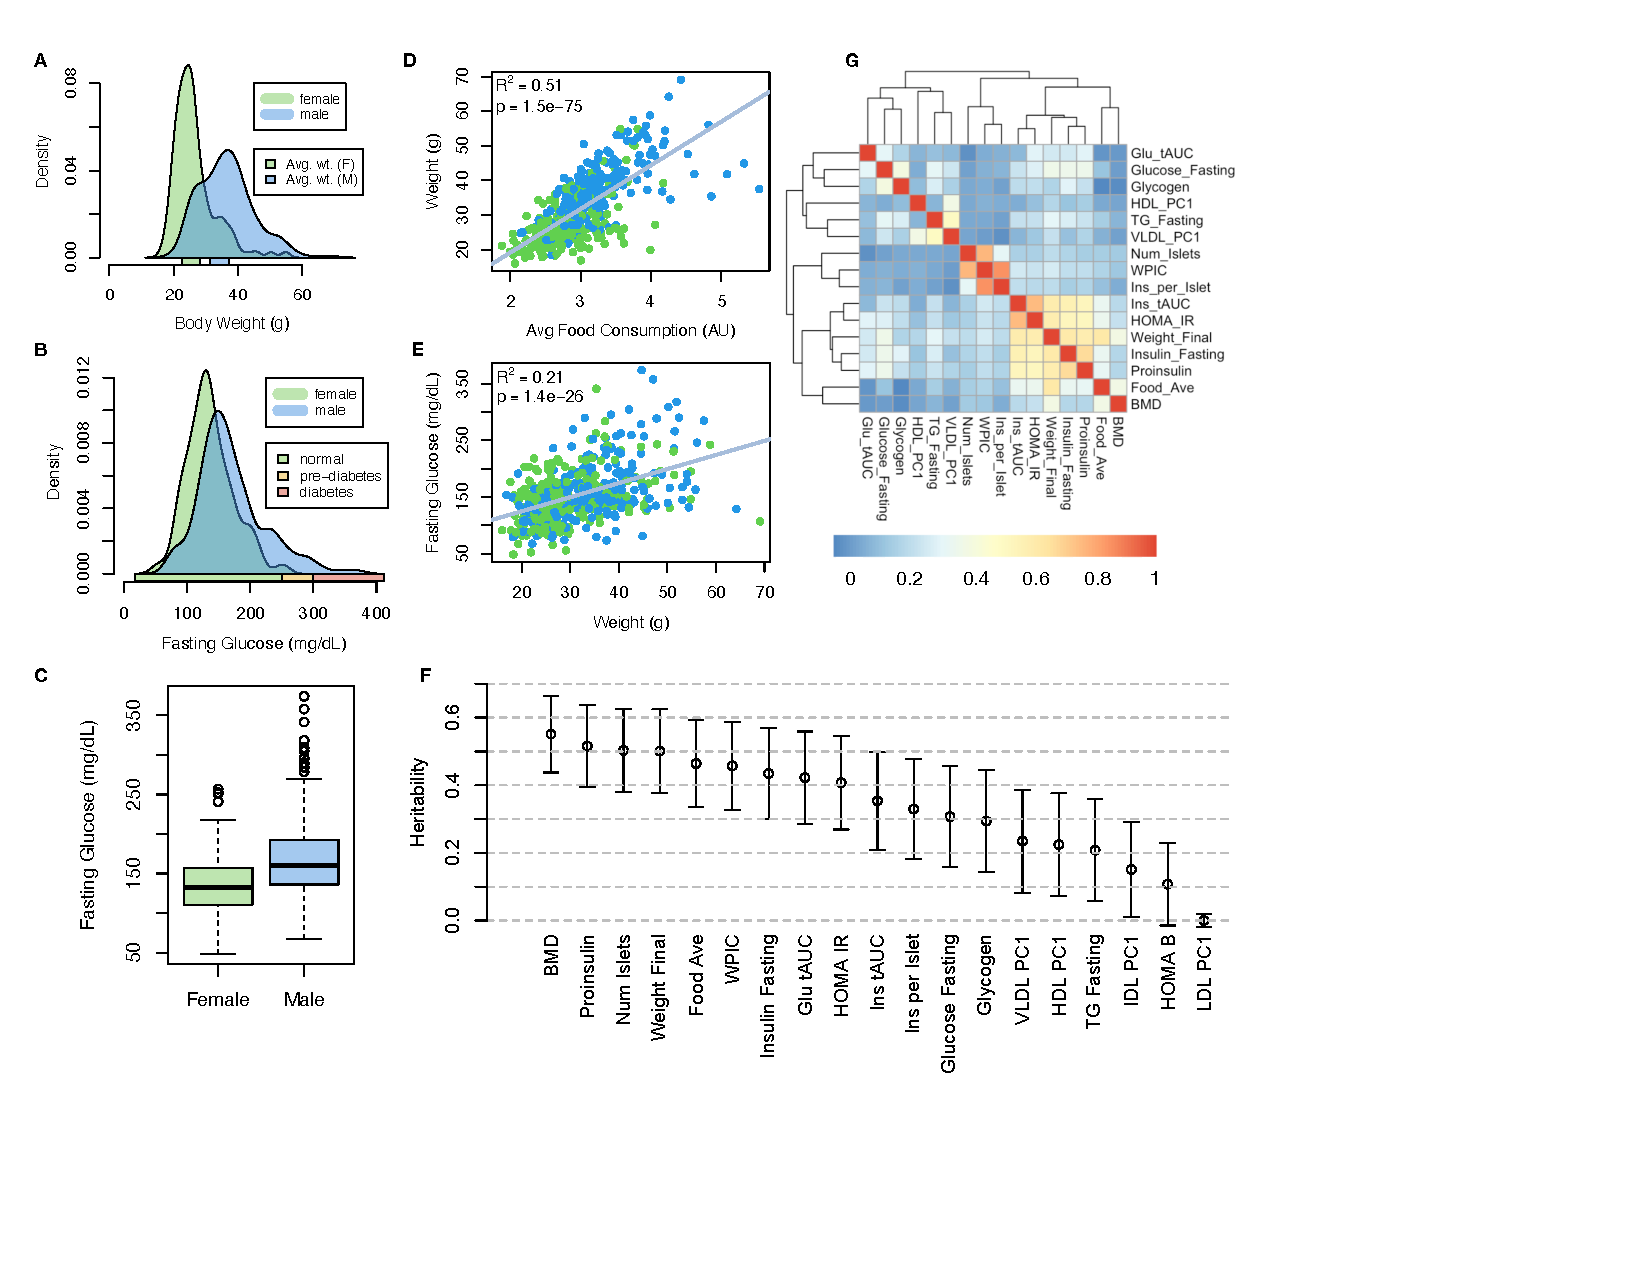
\includegraphics[width=\textwidth]{Figures/Fig1_trait_overview.pdf} 
\caption{Clinical overview. \textbf{A.} Distributions of final body weight 
in the diversity outbred mice. Sex is indicated by color. The 
average B6 male and female adult weights at 24 weeks of age 
are indicated by blue and green bars on the x-axis. \textbf{B.} The 
distribution of final fasting glucose across the population split 
by sex. Normal, pre-diabetic, and diabetic fasting glucose levels 
for mice are shown by colored bars along the x-axis. \textbf{C.} Males had 
higher fasting blood glucose on average than females. \textbf{D.} The 
relationship between food consumption and body weight for both 
sexes. \textbf{E.} Relationship between body weight and fasting glucose 
for both sexes. \textbf{F.} Heritability estimates for each physiological 
trait. Bars show standard error of the estimate. \textbf{G.} Correlation 
structure between pairs of physiological traits.}
\label{fig:trait_overview}
\end{figure}

The landscape of trait correlations (Fig. \ref{fig:trait_overview}G)
shows that most of the metabolic trait pairs were relatively weakly
correlated indicating complex relationships among the measured traits.
This low level of redundancy suggests a broad sampling of multiple
heritable aspects of metabolic disease including overall body weight,
glucose homeostasis, pancreatic composition and liver function.

\subsubsection{Distal Heritability Correlated with Phenotype
Relevance}\label{distal-heritability-correlated-with-phenotype-relevance}

We performed eQTL analysis using R/qtl2 \cite{pmid30591514} (Methods)
and identified both local and distal eQTL for transcripts in each of the
four tissues (Supp. Fig \ref{fig:eQTL}). Significant local eQTLs far
outnumbered distal eQTLs (Supp. Fig. \ref{fig:eQTL}F) and tended to be
shared across tissues (Supp. Fig. \ref{fig:eQTL}G) whereas the few
significant distal eQTL we identified tended to be tissue-specific
(Supp. Fig. \ref{fig:eQTL}H)

We calculated the heritability of each transcript in terms of local and
distal genetic factors (Methods). Overall, local and distal genetic
factors contributed approximately equally to transcript abundance. In
all tissues, both local and distal factors explained between 8 and 18\%
of the variance in the median transcript (Fig \ref{fig:motivation}A).

\begin{figure}[ht!]
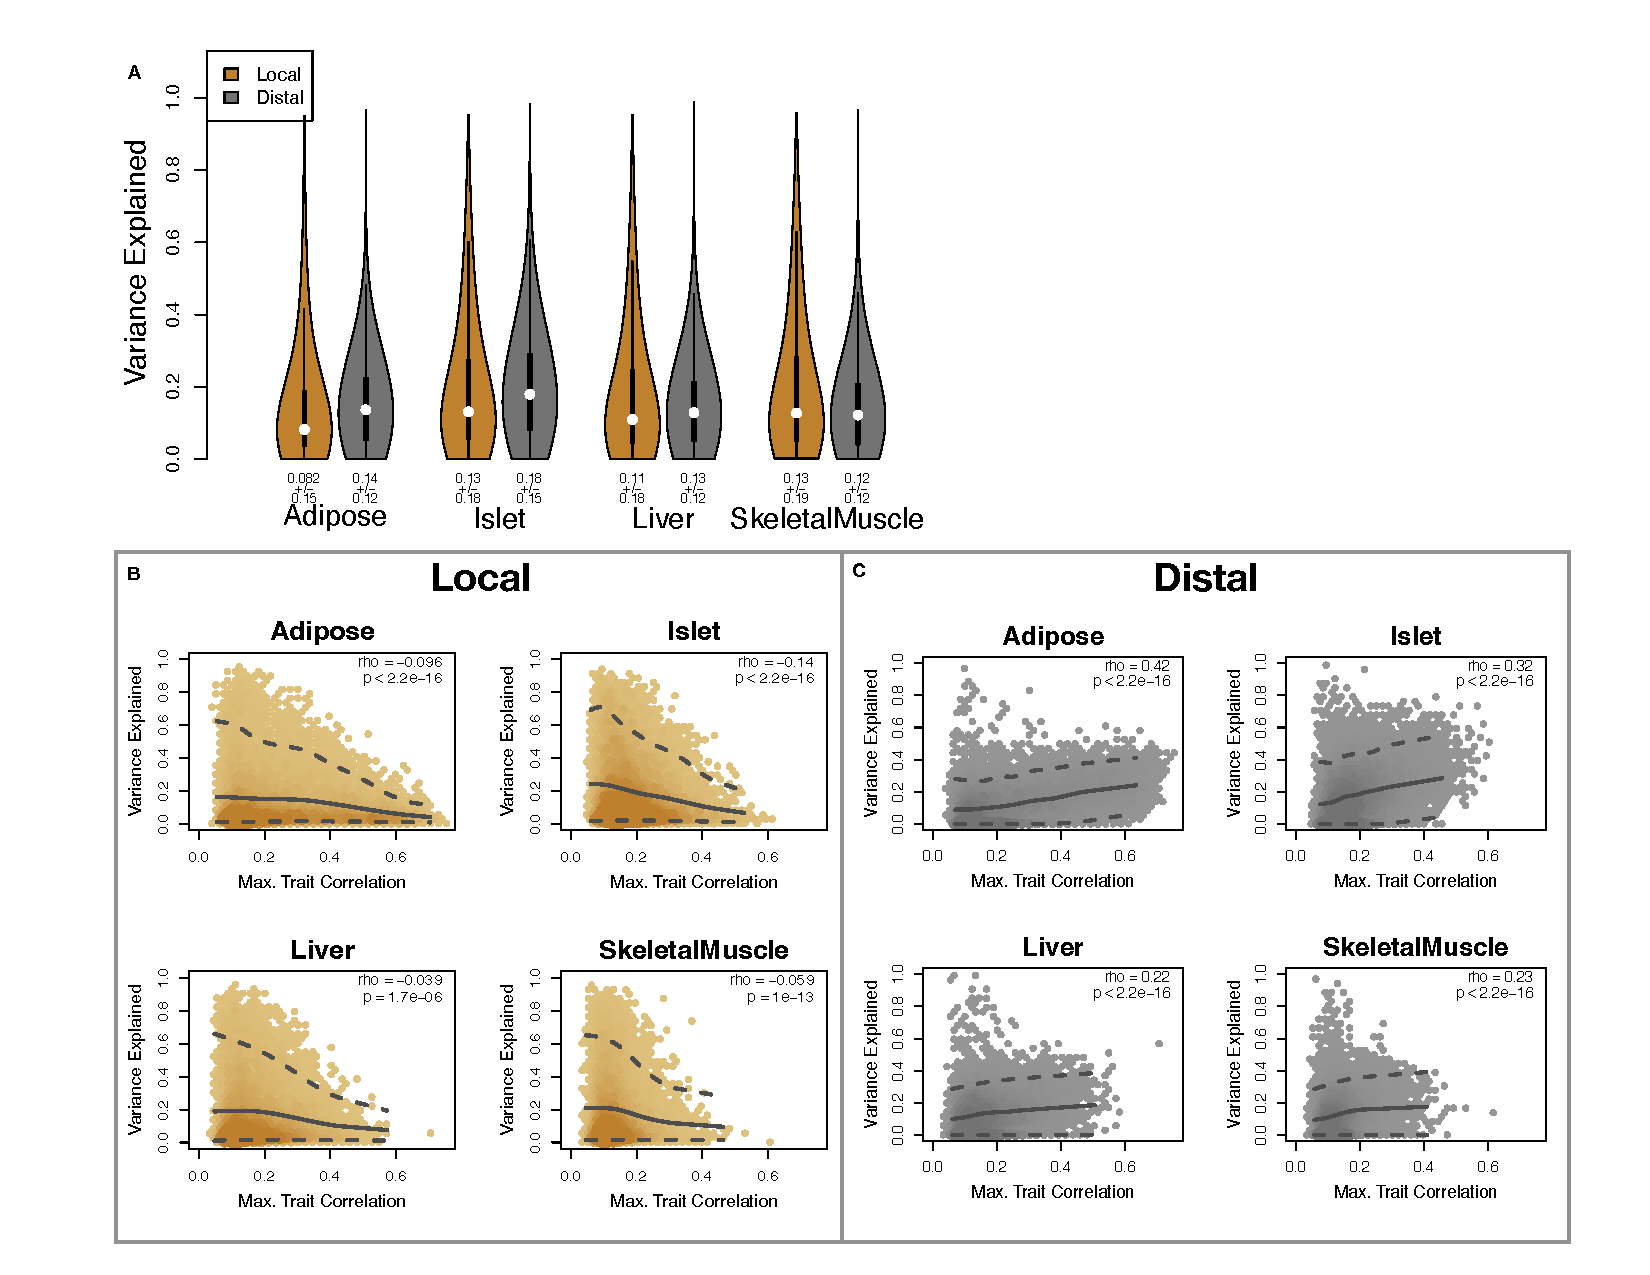
\includegraphics[width=\textwidth]{Figures/Fig2_motivation.pdf} 
\caption{Transcript heritability and trait relevance. 
\textbf{A.} Distributions of distal and local heritability of 
transcripts across the four tissues. Overall local and distal 
factors contribute equally to transcript heritability. The 
relationship between (\textbf{B.}) local and (\textbf{C.}) 
distal heritability and trait relevance across all four tissues. 
Here trait relevance is defined as the maximum correlation between 
the transcript and all traits. Local heritability was negatively 
correlated with trait relevance, and distal heritability is 
positively correlated with trait relevance. Pearson ($r$) and $p$ 
values for each correlation are shown in the upper-right of each panel.}
\label{fig:motivation}
\end{figure}

Local heritability of transcripts was negatively correlated with their
trait relevance, defined as the maximum correlation of a transcript
across all traits (Fig. \ref{fig:motivation}B). This suggests that the
more local genotype influenced transcript abundance, the less effect
variation in transcript abundance had on the measured traits.
Conversely, distal heritability of transcripts was positively correlated
with trait relevance (Fig. \ref{fig:motivation}C). That is, transcripts
that were more highly correlated with the measured traits tended to be
distally, rather than locally, heritable. That trait-correlated
transcripts have low local heritability is consistent with previous
observations that low-heritability transcripts explain more
expression-mediated disease heritability than high-heritability
transcripts \cite{pmid32424349}. However, the positive relationship
between trait correlation and distal heritability suggests that there
are alternative mechanisms through which genetic regulation of
transcripts may influence traits.

\subsubsection{High-Dimensional Mediation identified a high-heritability
composite trait that was perfectly mediated by a composite
transcript}\label{high-dimensional-mediation-identified-a-high-heritability-composite-trait-that-was-perfectly-mediated-by-a-composite-transcript}

We used high-dimensional mediation to identify the major axis of
variation in the transcriptome that mediated the effects of the genome
on metabolic traits (Fig. \ref{fig:workflow}). We kernelized the genome,
phenome, and transcriptome matrices and used generalized canonical
correlation analysis (RGCCA) \cite{rgcca} to identify a composite
transcript (\(T_C\)) that perfectly mediated the effect of the composite
genome (\(G_C\)) on the composite phenome (\(P_C\)).

\begin{figure}[ht!]
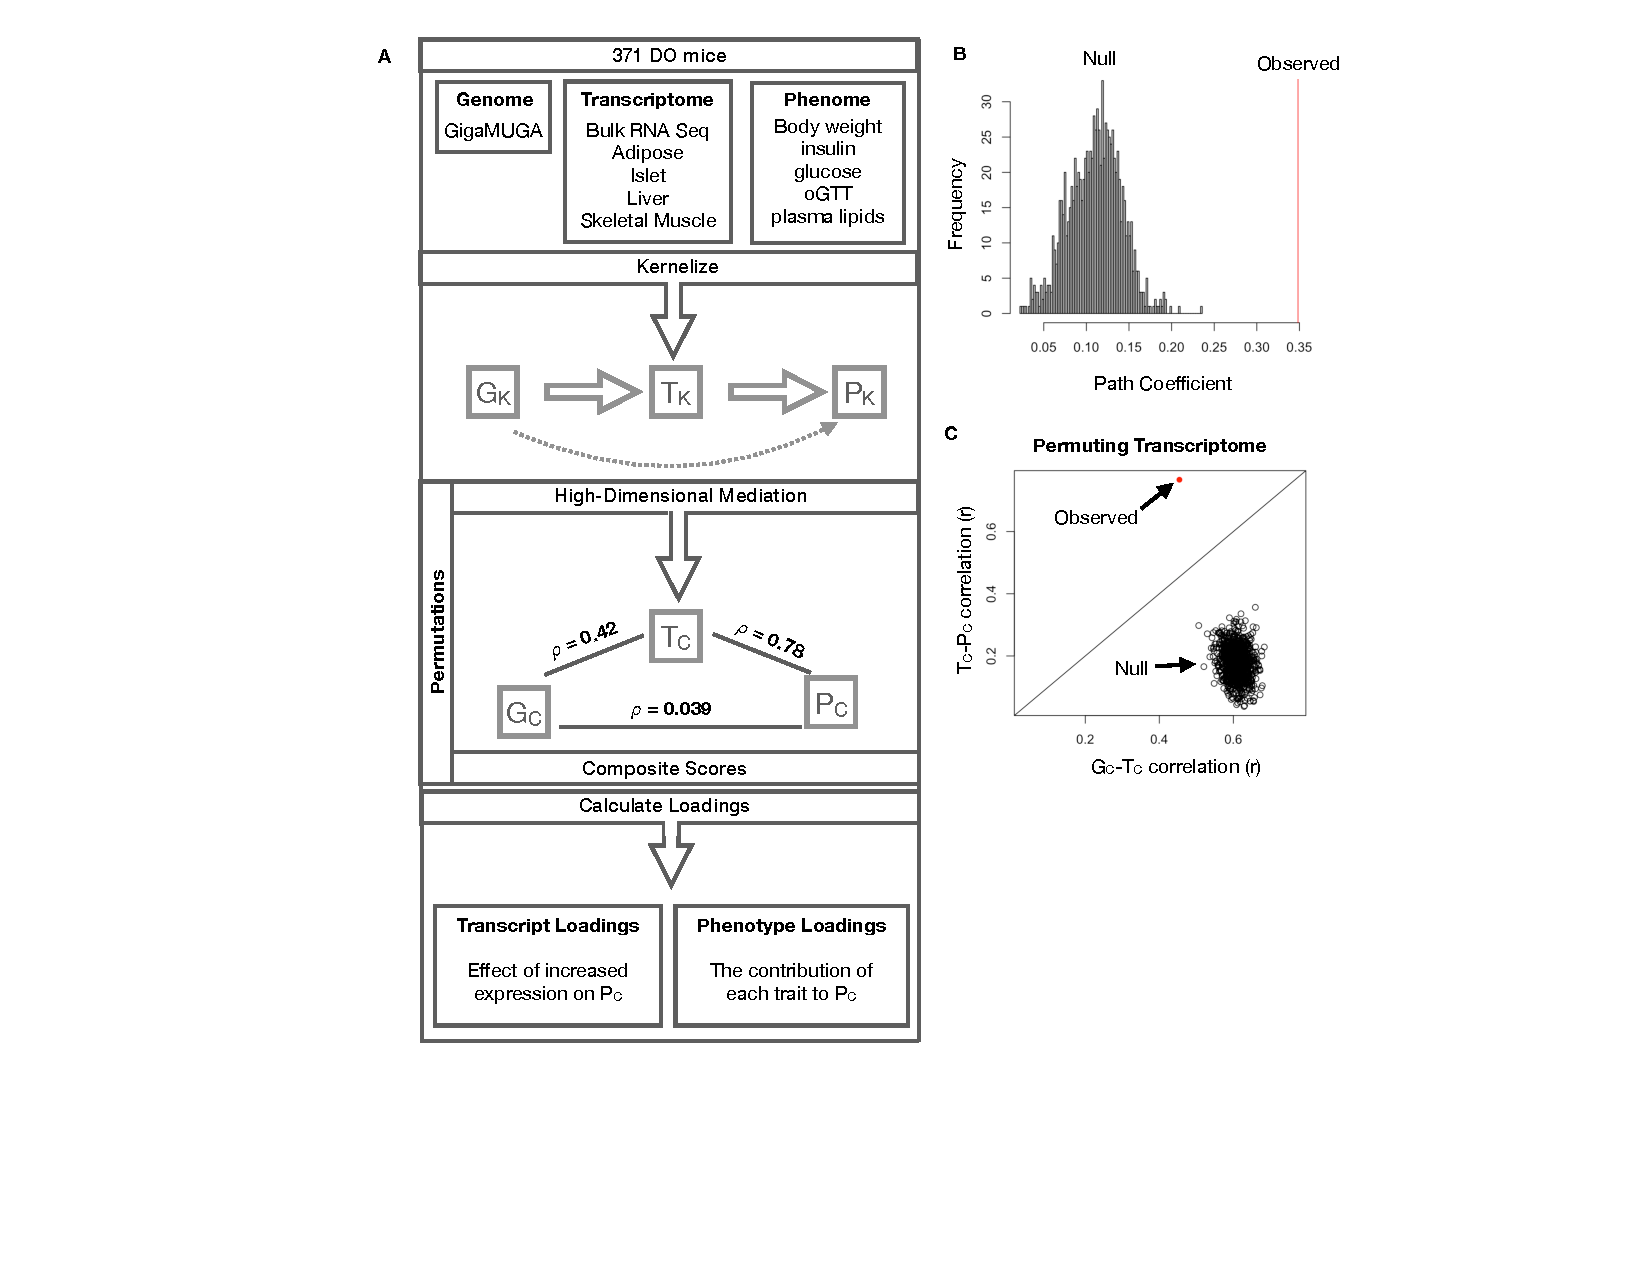
\includegraphics[width=5in]{Figures/Fig3_workflow.pdf} 
\caption{High-dimensional mediation. \textbf{A.} Workflow indicating 
major steps of high-dimensional mediation. The genotype, transcriptome, 
and phenotype matrices were kernelized to yield single matrices representing 
the relationships between all individuals for each data modality ($G_K$ = 
genome kernel, $T_K$ = transcriptome kernel; $P_K$ = phenome kernel). High-dimensional 
mediation was applied to these matrices to maximize the direct path 
$G \rightarrow T \rightarrow P$, the mediating pathway (arrows), while 
simultaneously minimizing the direct $G \rightarrow P$ pathway (dotted line). 
The composite vectors that resulted from high-dimensional mediation were 
$G_c$, $T_C$, and $P_C$. The partial correlations $\rho$ between these vectors 
indicated perfect mediation. Transcript and trait loadings were calculated 
as described in the methods. \textbf{B.} The null distribution of the path 
coefficient derived from 10,000 permutations compared to the observed path 
coefficient (red line). \textbf{C.} The null distribution of the $G_C$-$T_C$ 
correlation vs. the $T_C$-$P_C$ correlation compared with the observed value 
(red dot).
}
\label{fig:workflow}
\end{figure}

Fig. \ref{fig:workflow}A shows the partial correlations (\(\rho\))
between the pairs of these composite vectors. The partial correlation
between \(G_C\) and \(T_S\) was 0.42, and the partial correlation
between \(T_S\) and \(P_S\) was 0.78. However, when the transcriptome
was taken into account, the partial correlation between \(G_S\) and
\(P_S\) was effectively 0 (0.039). The estimated heritability of the
composite phenome was heritability of 0.71 \(\pm\) 0.084, which was
higher than any of the individual traits (Fig.
\ref{fig:trait_overview}F). Thus, we have identified a maximally
heritable metabolic trait that is perfectly mediated by a heritable
component of the transcriptome.

Standard CCA is prone to over-fitting because in any two large matrices
it can be trivial to identify highly correlated composite vectors. To
assess whether RGCCA was similarly prone to over-fitting in a
high-dimensional space, we performed permutation testing. We permuted
the individual labels on the transcriptome kernel matrix 1000 times and
recalculated the path coefficient, which is the partial correlation of
\(G_C\) and \(T_C\) multiplied by the partial correlation of \(T_C\) and
\(P_C\). This represents the path from \(G_C\) to \(P_C\) that is
mediated through \(T_C\). The null distribution of the path coefficient
is shown in Fig. \ref{fig:workflow}B, and the observed path coefficient
from the original data is indicated by the red line. The observed path
coefficient was well outside the null distribution generated by
permutations. Fig. \ref{fig:workflow}C illustrates this observation in
more detail. Although we identified high correlations between \(G_C\)
and \(T_C\), and modest correlations between \(T_C\) and \(P_C\) in the
null data (Fig \ref{fig:workflow}C), these two values could not be
maximized simultaneously. The red dot shows that in the real data both
the \(G_C\)-\(T_C\) correlation and the \(T_C\)-\(P_C\) correlation
could be maximized simultaneously suggesting that the path from genotype
to phenotype through transcriptome is highly non-trivial and
identifiable in this case. These results suggest that these composite
vectors represent genetically determined variation in phenotype that is
mediated through genetically determined variation in transcription.

\subsubsection{Body weight and insulin resistance were highly
represented in the expression-mediated composite
trait}\label{body-weight-and-insulin-resistance-were-highly-represented-in-the-expression-mediated-composite-trait}

The loadings of each measured trait onto \(P_C\) indicate how much each
contributed to the composite phenotype. Final body weight contributed
the most (Fig. \ref{fig:interpretation}), followed by homeostatic
insulin resistance (HOMA\_IR) and fasting plasma insulin levels
(Insulin\_Fasting). We can thus interpret \(P_C\) as an index of
metabolic disease (Fig. \ref{fig:interpretation}B). Individuals with
high values of \(P_C\) have a higher metabolic index and greater
metabolic disease, including higher body weight and higher insulin
resistance. We refer to \(P_C\) as the metabolic index going forward.
Traits contributing the least to the metabolic index were measures of
cholesterol and pancreas composition. Thus, when we interpret the
transcriptomic signature identified by HDM, we are explaining primarily
transcriptional mediation of body weight and insulin resistance, as
opposed to cholesterol measurements.

\begin{figure}[ht!]
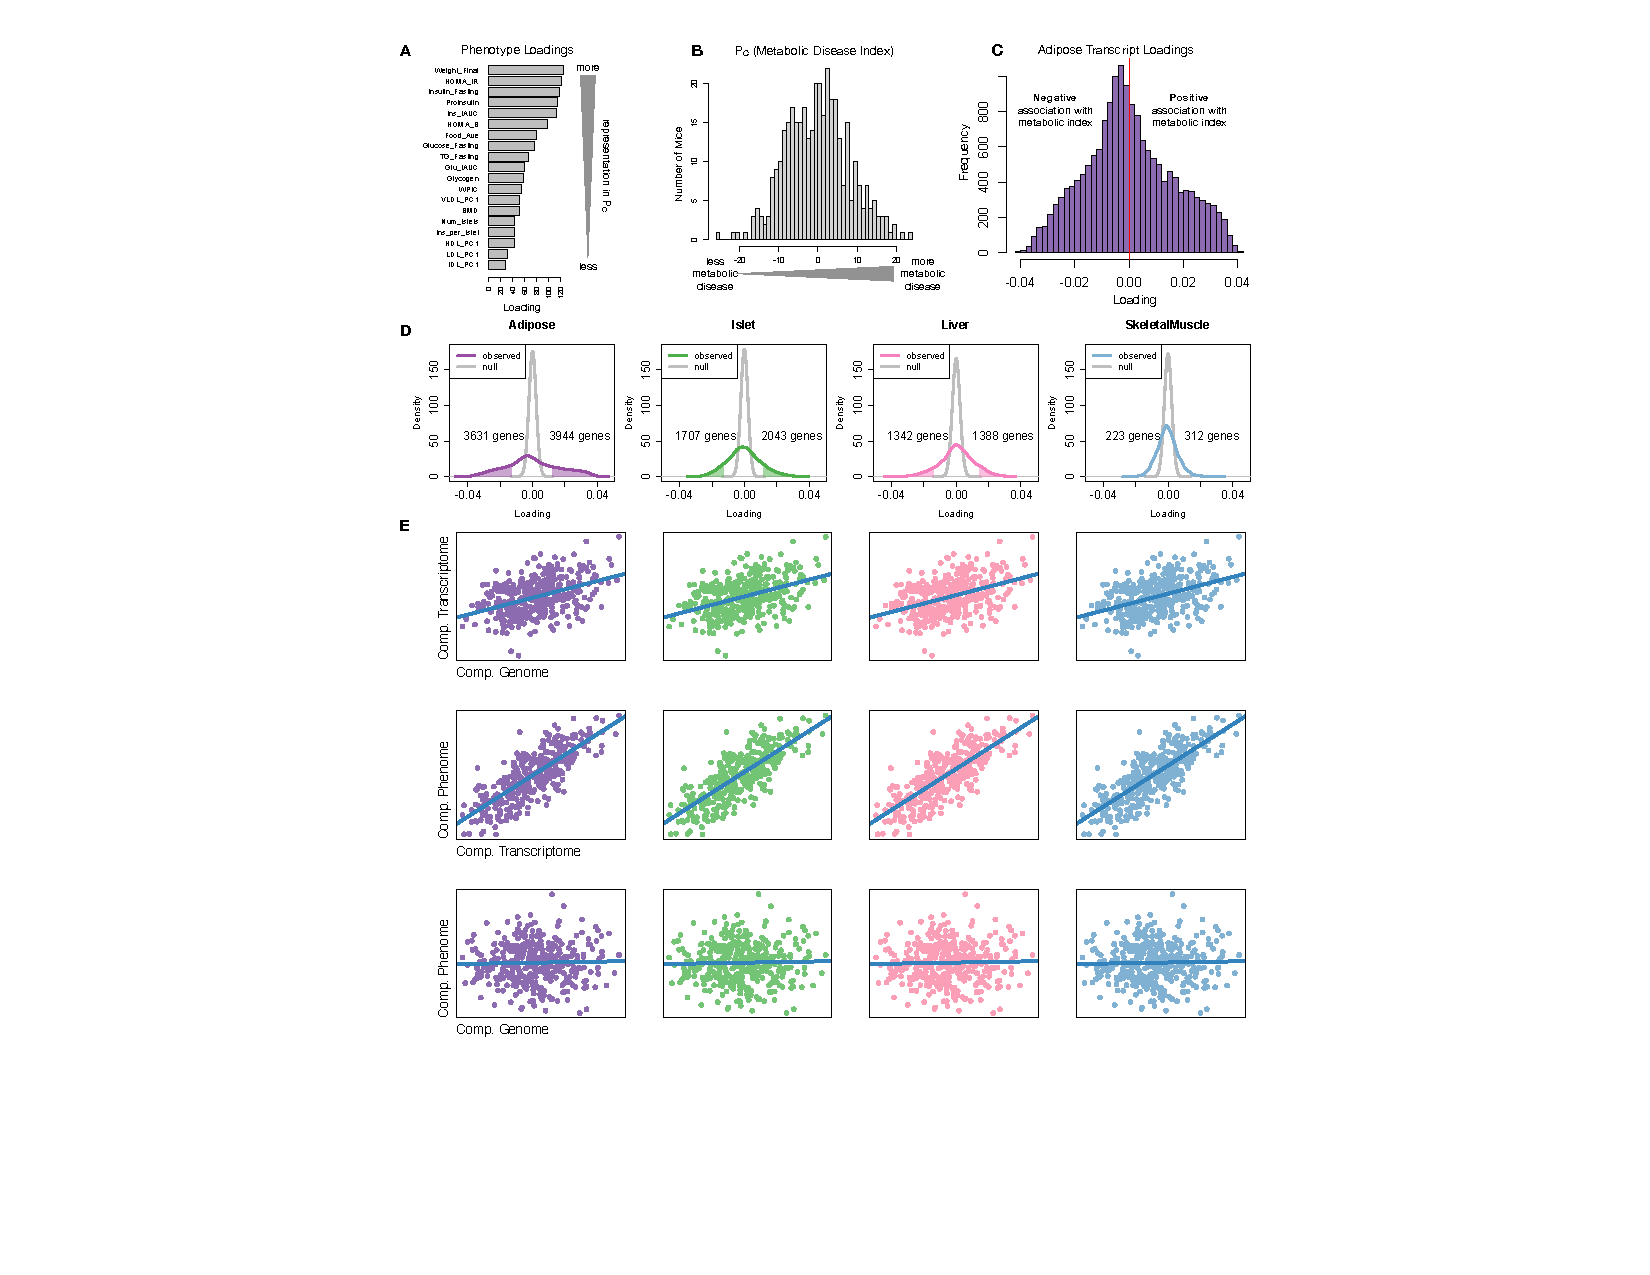
\includegraphics[width=\textwidth]{Figures/Fig4_interpretation.pdf} 
\caption{Interpretation of loadings. \textbf{A.} Loadings 
across traits. Body weight and insulin resistance contributed 
the most to the composite trait. \textbf{B.} Phenotype scores 
across individuals. Individuals with large positive phenotype 
scores had higher body weight and insulin resistance than average. 
Individuals with large negative phenotype scores had lower body 
weight and insulin resistance than average. \textbf{C.} 
Distribution of transcript loadings in adipose tissue. For 
transcripts with large positive loadings, higher expression was 
associated with higher phenotype scores. For transcripts with 
large negative loadings, higher expression was associated with 
lower phenotype scores. \textbf{D.} Distribution of absolute 
value of transcript loadings across tissues. Transcripts in 
adipose tissue had the largest loadings indicating that 
transcripts in adipose tissue were the best mediators of the 
genetic effects on body weight and insulin resistance.
}
\label{fig:interpretation}
\end{figure}

\subsubsection{High-loading transcripts have low local heritability,
high distal heritability, and were linked mechanistically to
obesity}\label{high-loading-transcripts-have-low-local-heritability-high-distal-heritability-and-were-linked-mechanistically-to-obesity}

We interpreted large loadings onto transcripts as indicating strong
mediation of the effect of genetics on metabolic index. Large positive
loadings indicate that higher expression was associated with a higher
metabolic index (i.e.~higher risk of obesity and metabolic disease on
the high-fat diet) (Fig. \ref{fig:interpretation}C). Conversely, large
negative loadings indicate that high expression of these transcripts was
associated with a lower metabolic index (i.e.~lower risk of obesity and
metabolic disease on the high-fat diet) (Fig.
\ref{fig:interpretation}C). We used gene set enrichment analysis (GSEA)
\cite{fgsea, 
pmid16199517} to look for biological processes and pathways that were
enriched at the top and bottom of this list (Methods).

In adipose tissue, both GO processes and KEGG pathway enrichments
pointed to an axis of inflammation and metabolism (Supp. Fig.
\ref{fig:top_enrich_kegg} and \ref{fig:top_enrich_go}). GP terms and
KEGG pathways associated with inflammation, particularly macrophage
infiltration, were positively associated with metabolic index,
indicating that increased expression in inflammatory pathways was
associated with a higher metabolic index. It is well established that
adipose tissue in obese individuals is highly inflamed {[}cite{]} and
infiltrated by macrophages {[}cite{]}, and the results here suggest that
this may be a heritable component of metabolic disease.

The strongest negative enrichments in adipose tissue were related to
mitochondial activity in general, and thermogenesis in particular (Supp.
Fig. \ref{fig:top_enrich_kegg} and \ref{fig:top_enrich_go}). It has been
shown mouse strains with greater thermogenic potential are also less
susceptible to obesity on a high-fat diet {[}cite{]}.

Transcripts associated with the citric acid (TCA) cycle as well as the
catabolism of branched-chain amino acids (BCAA), valine, leuceine, and
isoleucine were strongly enriched with negative loadings in adipose
tissue (Supp. Fig. XXX). Expression of genes in both pathways (for which
there is some overlap) has been previously associated with insulin
sensitivity \cite{pmid29567659, 
pmid22560213, pmid19841271}, suggesting that heritable variation in
regulation of these pathways may influence risk of insulin resistance.

Looking a the 10 strongest positive and negative loaded transcripts from
each tissue, is is apparent that transcripts in the adipose tissue had
the largest loadings, both positive and negative, of all tissues (Fig.
\ref{fig:loading_heritability}A bar plot) This suggesting that much of
the effect of genetics on body weight and insulin reisistance is
mediated through gene expression in adipose tissue. The strongest
loadings in liver and pancreas were comparable, and those in skeletal
muscle were the weakest (Fig. \ref{fig:loading_heritability}A),
suggesting that less of the genetic effects were mediated through
transcription in skeletal muscle. Heritability analysis showed that
trahscripts with the largest loadings tended to have relatively high
distal heritability compared with local heritability (Fig.
\ref{fig:loading_heritability}A heat map and box plot). This pattern
contrasts with transcripts nominated by TWAS (Fig.
\ref{fig:loading_heritability}B), which tended to have lower loadings,
higher local heritability and lower distal heritability. Transcripts
with the highest local heritability in each tissue (Fig.
\ref{fig:loading_heritability}C) had the lowest loadings.

We performed a literature search for the genes in each of these groups
along with the terms ``diabetes'', ``obesity'', and the name of the
expressing tissue to determine whether any of these genes had previous
associations with metabolic disease in the literature (Methods).
Multiple genes in each group had been previously associated with obesity
and diabetes (Fig. \ref{fig:loading_heritability} bolded gene names).
Genes with high loadings were most highly enriched for previous
literature support. They were 2.25 more likely than TWAS hits and 3.6
times more likely than genes with high local heritability to be
previously associated with obesity or diabetes.

\begin{figure}[ht!]
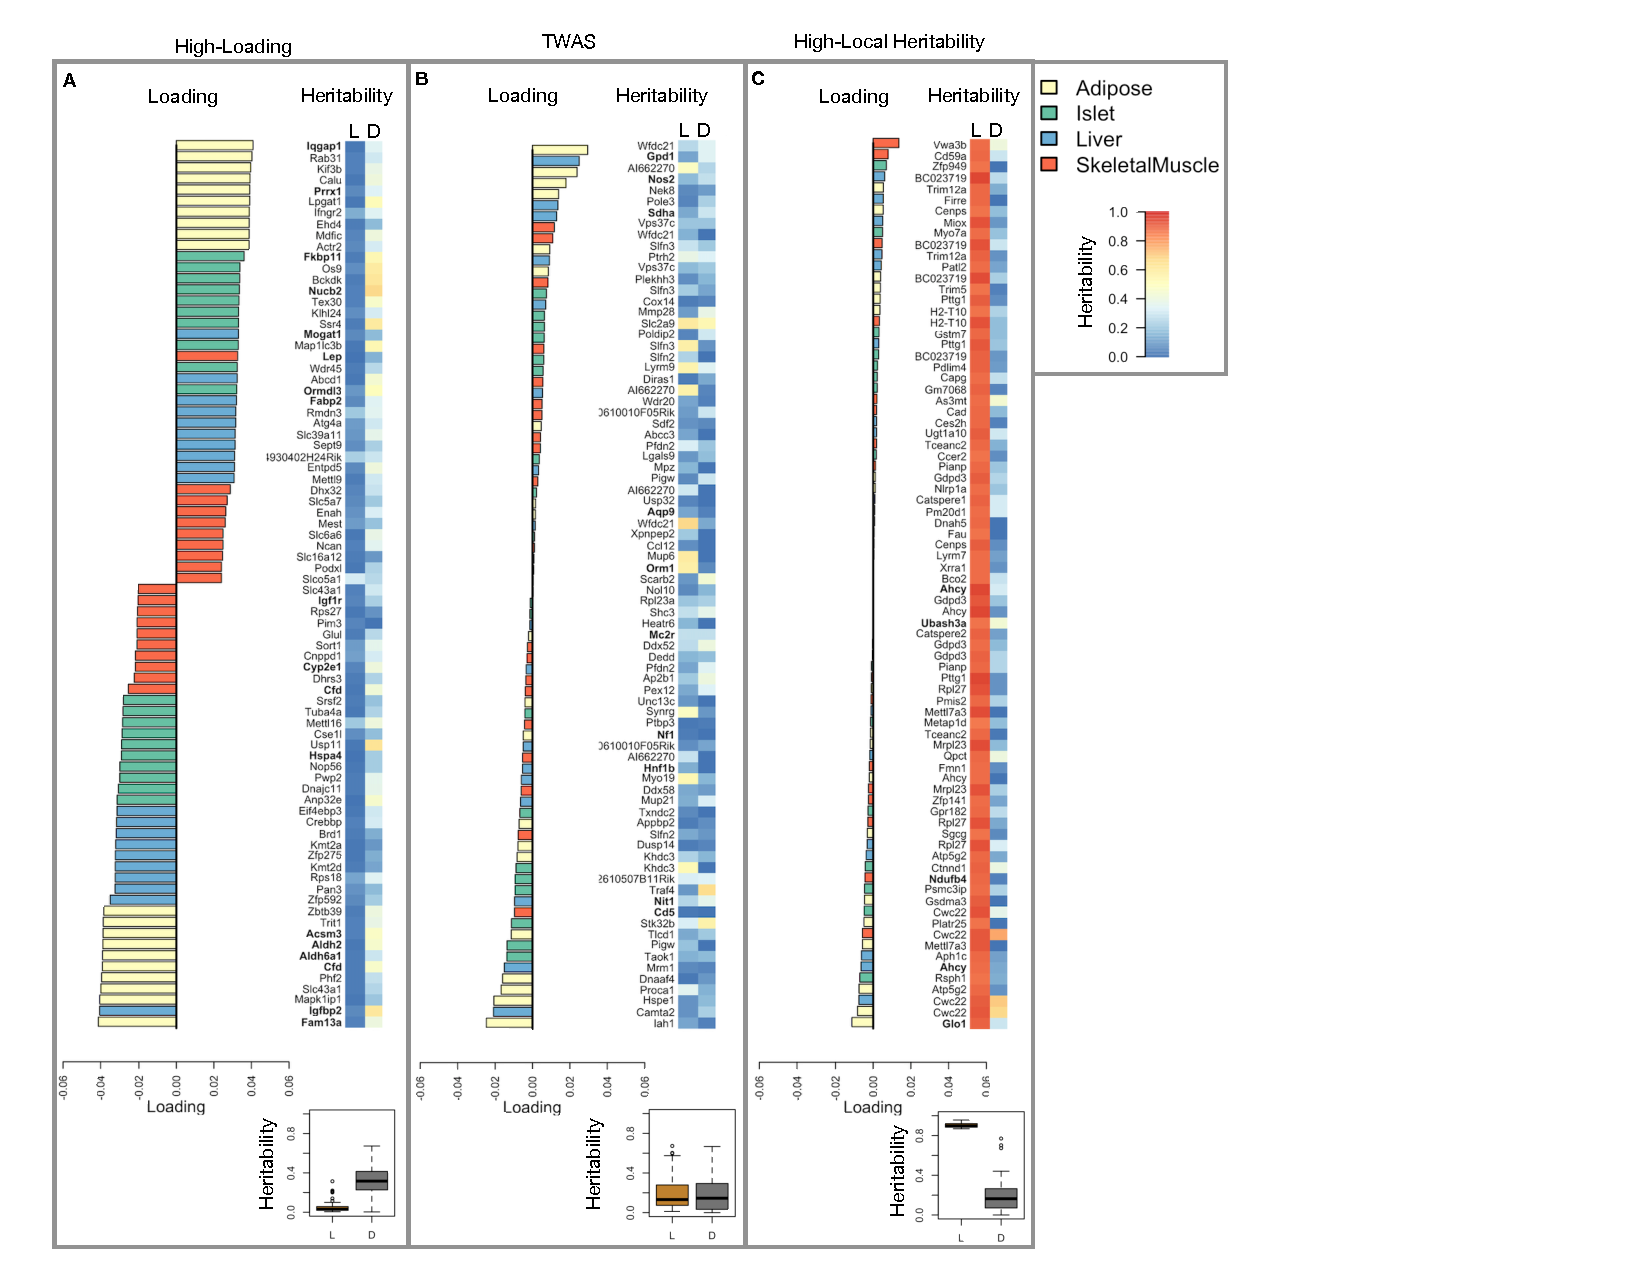
\includegraphics[width=\textwidth]{Figures/Fig5_loading_heritability.pdf} 
\caption{Transcripts with high loadings have high distal heritability
and literature support. Each panel has a bar plot showing the loadings 
of transcripts selected by different criteria. Bar color indicates the 
tissue of origin. The heat map shows the local (L - left) and distal 
(D - right) heritability of each transcript. \textbf{A.} Loadings for 
the 10 transcripts with the largest positive loadings and the 10 
transcripts with the largest negative loadings for each tissue. 
\textbf{B.} Loadings of TWAS candidates with the 10 largest positive 
correlations with traits and the largest negative correlations with 
traits across all four tissues. \textbf{C.} The transcripts with the 
largest local heritability (top 20) across all four tissues.
}
\label{fig:loading_heritability}
\end{figure}

\subsubsection{Tissue-specific transriptional programs were associated
with metabolic
traits}\label{tissue-specific-transriptional-programs-were-associated-with-metabolic-traits}

Clustering of transcripts with top loadings in each tissue showed
tissue-specific functional modules associated with obesity and insulin
resistance (Fig. \ref{fig:toa}A) (Methods). The clustering highlights
the importance of immune activation particularly in adipose tissue.
Except fo the ``mitosis'' cluster, which had large positive loadings in
three of the four tissues, all clusters were strongly loaded in only one
or two tissues. For example, the lipid metabolism cluster was loaded
most heavily in liver. The positive loadings suggest that high
expression of these genes particualarly in the liver was associated with
increased metabolic disease. This cluster included the gene
\textit{Pparg}, whose primary role is in the adipose tissue where it is
considered a master regulator of adipogenesis \cite{pmid17389767}.
Agonists of \textit{Pparg}, such as Thiazolidinediones, which are
FDA-approved to treat type II diabetes, reduce inflammation and adipose
hyptertrophy \cite{pmid17389767}. Consistent with this role, the loading
for \textit{Pparg} in adipose tissue was negative, suggesting that
higher expression was associated with leaner mice (Fig. \ref{fig:toa}B).
In contrast, \textit{Pparg} had a large positive loading in liver, where
it is known to play a role in the development of hepatic steatosis, or
fatty liver. Mice that lack \textit{Pparg} specifically in the liver,
are protected from developing steatosis and show reduced expression of
lipogenic genes \cite{pmid12805374, pmid12618528}. Overexpression of
\textit{Pparg} in the livers of mice with a \textit{Ppara} knockout,
causes upregulation of genes involved in adipogenesis
\cite{pmid16357043}. In the livers of both mice and humans high
\textit{Pparg} expression is associated with hepatocytes that accumulate
large lipid droplets and have gene expression profiles similar to
adipocytes \cite{pmid15644454, pmid16403437}.

The local and distal heritability of \textit{Pparg} is low in adipose
tissue suggesting its expression in this tissue is highly constrained in
the population (Fig. \ref{fig:toa}B). However, the distal heritability
of \textit{Pparg} in liver is relatively high suggesting it is complexly
regulated and has sufficient variation in this population to drive
variation in phenotype. Both local and distal heribatility of
\textit{Pparg} in the islet are fairly high, but the loading is low,
suggesting that variability of expression in the islet does not drive
phenotypic variation. These results highlight the importance of tissue
context when investigating the role of heritable transcript variability
in driving phenotype.

Gene lists for all clusters are available in Supplemental File XXX.

\begin{figure}[ht!]
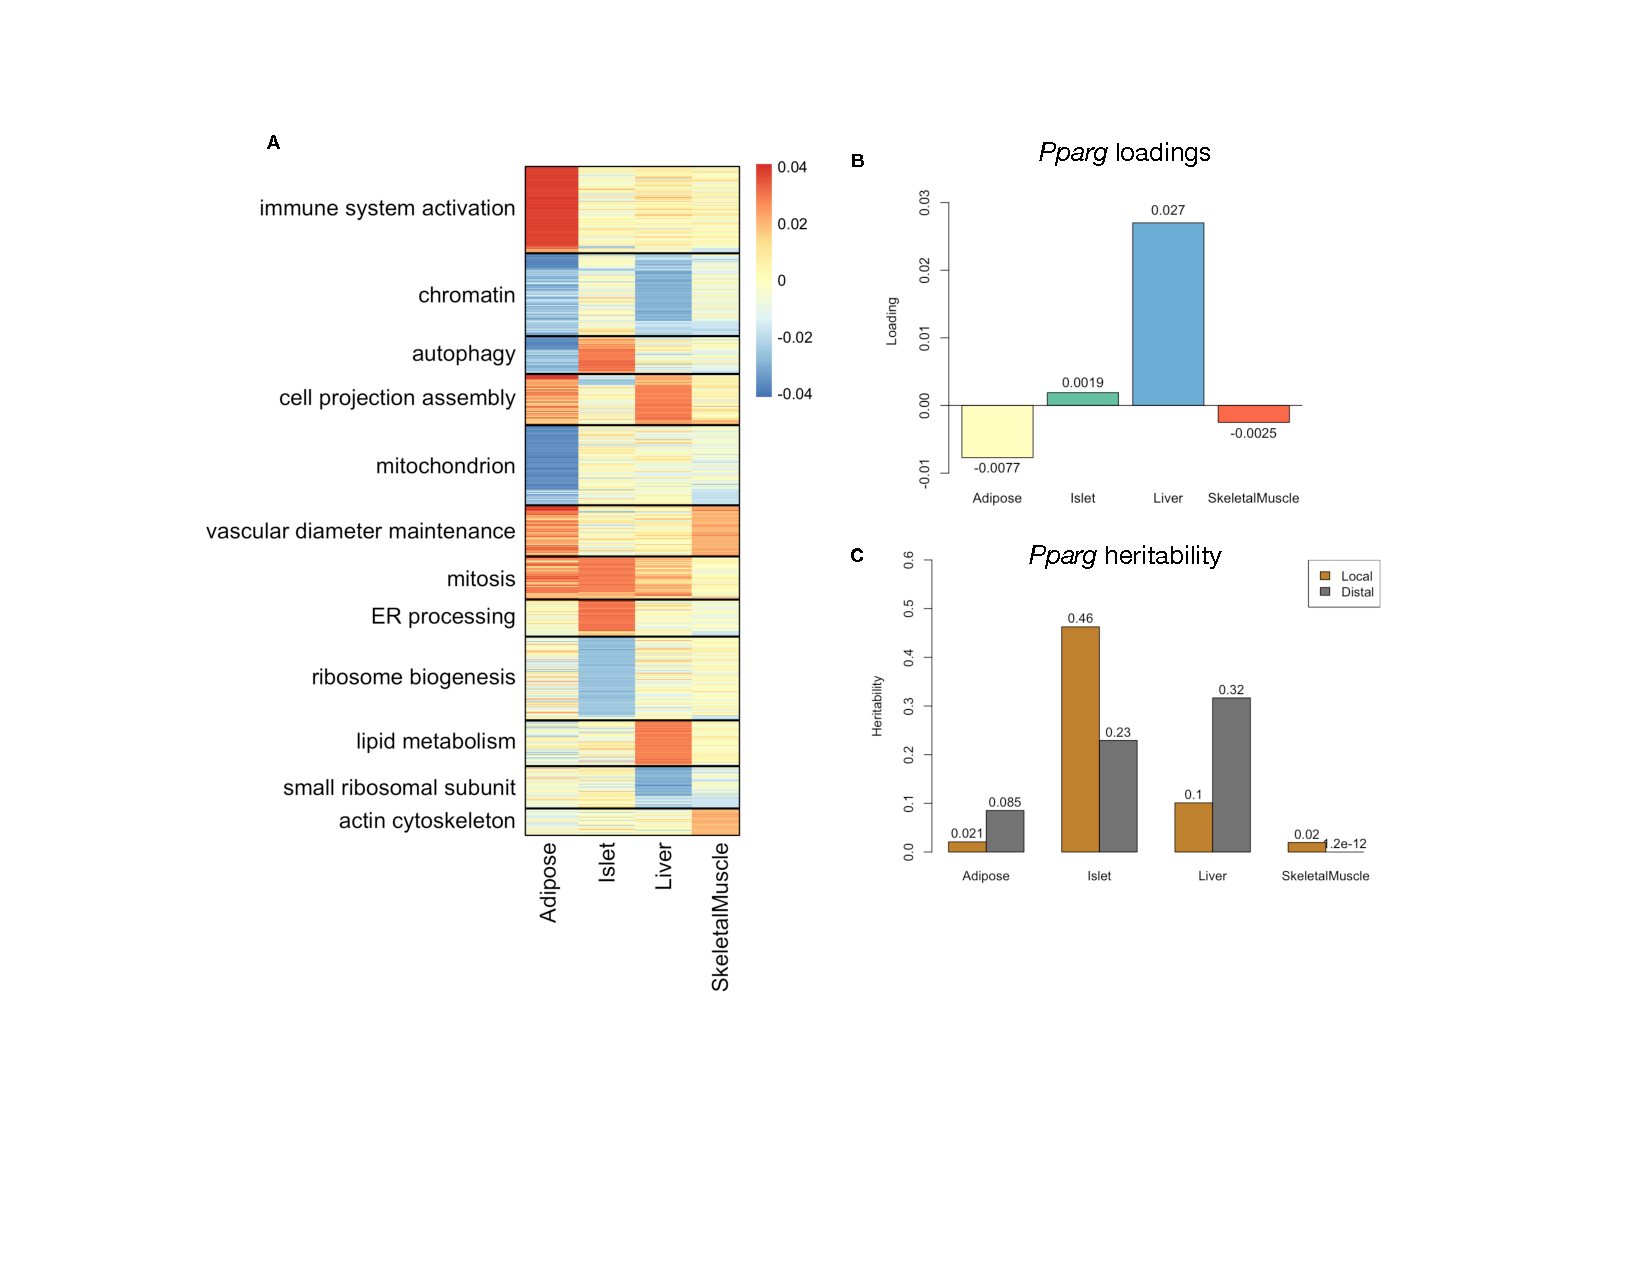
\includegraphics[width=\textwidth]{Figures/Fig6_TOA.pdf} 
\caption{Tissue-specific transcriptional programs were associated 
with obesity and insulin resistance. \textbf{A} Heat map showing 
the loadings of all transcripts with loadings greater than 2.5 
standard deviations from the mean in any tissue. The heat map was 
clustered using k medoid clustering. Functional enrichments of each 
cluster are indicated along the left margin. \textbf{B} Loadings for 
\textit{Pparg} in different tissues. \textbf{C} Local and distal of 
\textit{Pparg} expression in different tissues.
}
\label{fig:toa}
\end{figure}

\subsubsection{Gene expression, but not local eQTLs, predicted body
weight in an independent
population}\label{gene-expression-but-not-local-eqtls-predicted-body-weight-in-an-independent-population}

To test whether the transcript loadings identified in the DO could be
translated to another population, we tested whether they could predict
metaoblic a phenotype in an independent population of CC-RIX mice, which
were F1 mice derived from multiple pairings of Collaborative Cross (CC)
{[}cite{]} strains (Fig. \ref{fig:cc_prediction}) (Methods). We tested
two questions. First, we asked whether the loadings identified in the DO
mice were relevant to the relationship between the transcriptome and the
phenome in the CC-RIX. We predicted body weight in each CC-RIX
individual using measured gene expression in each tissue and the
transcript loadings identified in the DO (Methods). The predicted body
weight and acutal body weight were highly correlated in all tissues
(Fig. \ref{fig:cc_prediction}B left column). The best prediction was
achieved for adipose tissue, which supports the observation in the DO
that adipose expression was the strongest mediator of the genetic effect
on metabolic index. This result also confirms the validity and
translatability of the transcript loadings and their relationship to
metabolic disease.

\begin{figure}[ht!]
\includegraphics[width=\textwidth]{Figures/Fig7_CC_Prediction.pdf} 
\caption{Transcription, but not local genotype, predicts 
phenotype in the CC-RIX. \textbf{A.} Workflow showing procedure 
for translating HDM results to an independent population of mice. 
\textbf{B.} Relationships between the predicted metabolic index 
and measured body weight. The left column shows the predictions 
using measured transcripts. The right column shows the prediction 
using transcript levels imputed from local genotype. Gray boxes 
indicate measured quantities, and blue boxes indicate calculated 
quantities. The dots in each panel represent individual CC-RIX strains. 
The gray lines show the standard deviation on body weight for the strain.
}
\label{fig:cc_prediction}
\end{figure}

The second question related to the source of the relevant variation in
gene expression. If local regulation was the predominant factor
influencing gene expression, we should be able to predict phenotype in
the CC-RIX using transcripts imputed from local genotype (Fig.
\ref{fig:cc_prediction}A). The DO and the CC-RIX were derived from the
same eight founder strains and so carry the same alleles throughout the
genome. We imputed gene expression in the CC-RIX using local genotype
and were able to estimate variation in gene transcription robustly
(Supp. Fig. \ref{fig:cc_imputation}). However, these imputed values
failed to predict body weight in the CC-RIX when weighted with the
loadings from HDM. (Fig. \ref{fig:cc_prediction}B right column). This
result suggests that local regulation of gene expression is not the
primary factor driving heritability of complex traits.

\subsubsection{Distally heritable transcriptomic signatures reflected
variation in composition of adipose tissue and
islets}\label{distally-heritable-transcriptomic-signatures-reflected-variation-in-composition-of-adipose-tissue-and-islets}

Interpretation of global genetic influences on gene expression and
phenotype is potentially more challenging than interpretation and
translation of local genetic influences, as genetic effects cannot be
localized to individual gene variants or transcripts. However, there are
global patterns across the loadings that can inform mechanism. For
example, heritable variation in cell type composition can be derived
from transcript loadings. We noted earlier that immune activation in the
adipose tissues was an important driver of obesity in the DO population.
To determine whether this is reflected as an increase in macrophages in
adipose tissue, we compared loadings of cell-type specific genes in
adipose tissue (Methods). The mean loading of macrophage-specific genes
was substantially greater than 0 (Fig. \ref{fig:human_translation}A),
indicating that obese mice were genetically predisposed to have high
levels of macrophage infiltration in adipose tissue in response to the
high-fat, high-sugar diet.

\begin{figure}[ht!]
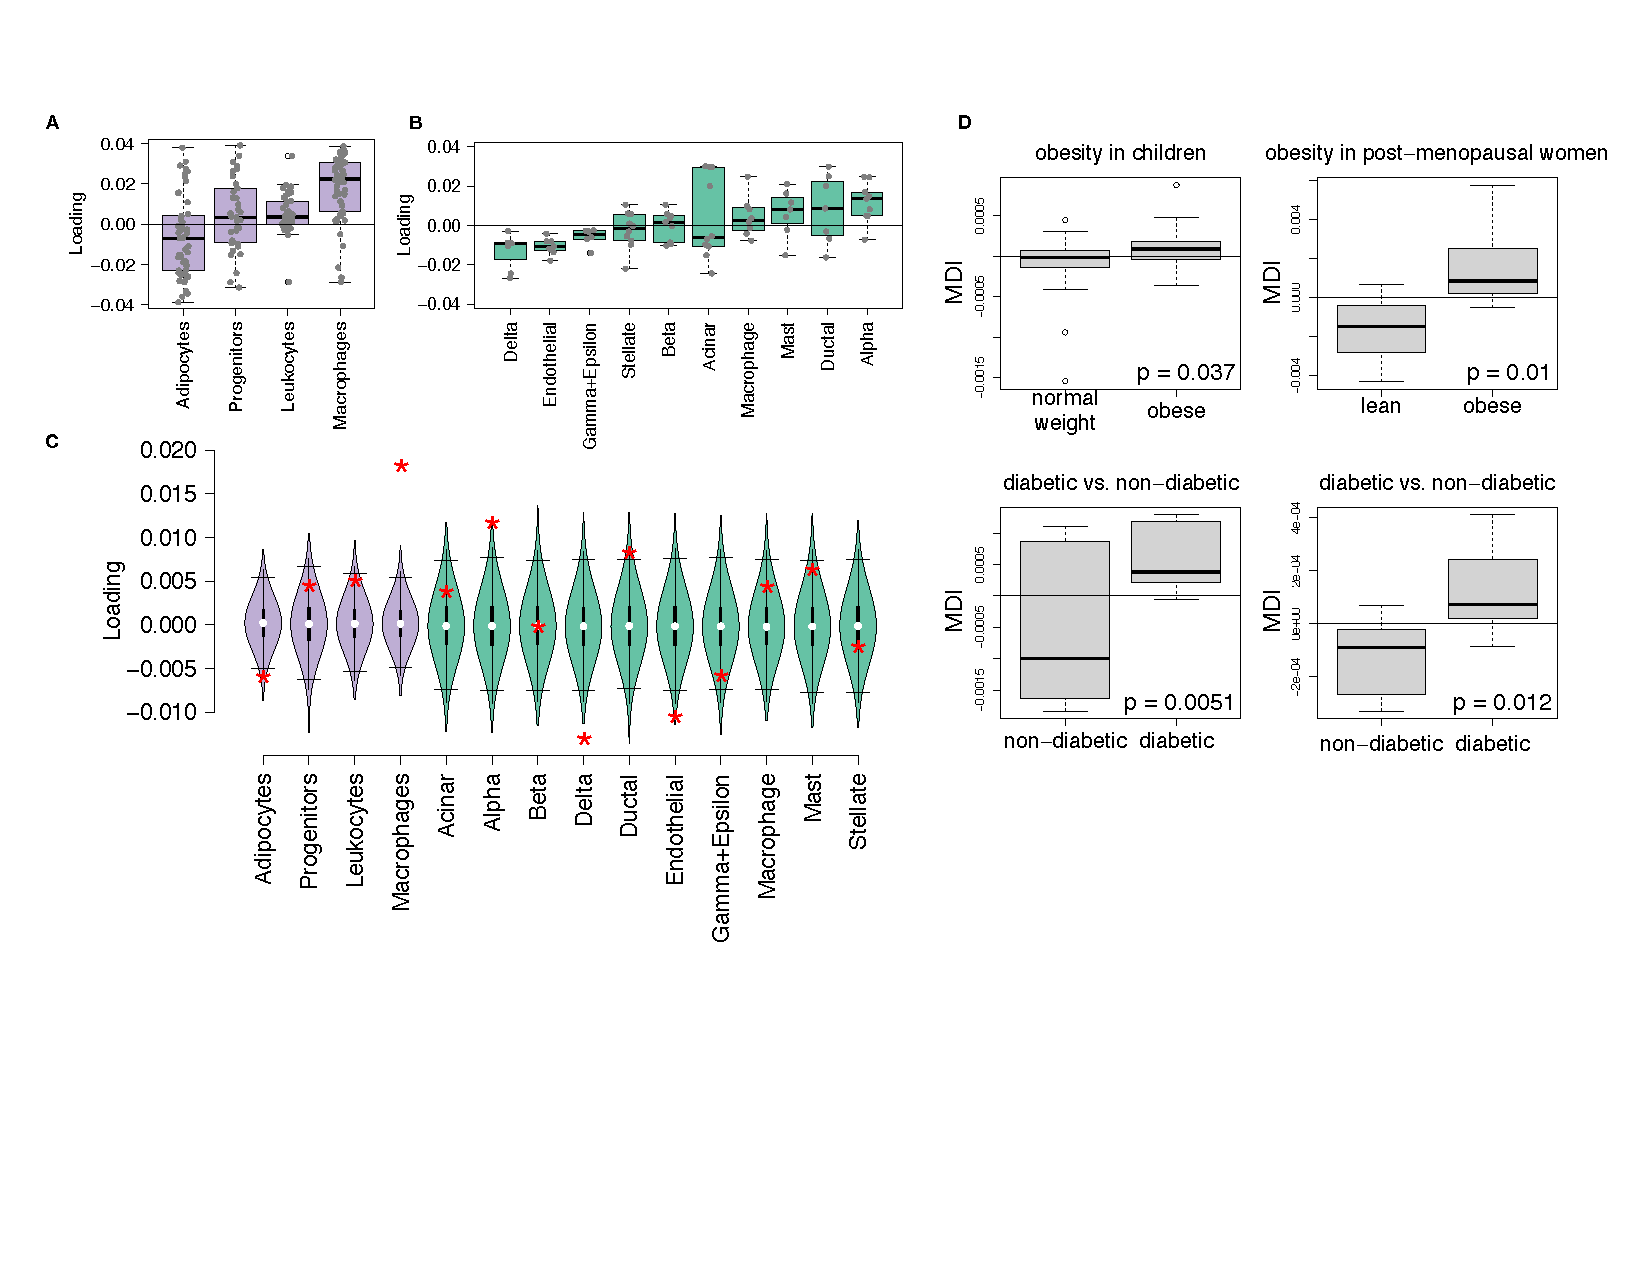
\includegraphics[width=\textwidth]{Figures/Fig8_Human_Translation.pdf} 
\caption{HDM results translate to humans. \textbf{A.} Distribution of 
loadings for cell-type-specific transcripts in adipose tissue. \textbf{B.} 
Distribution of loadings for cell-type-specific transcripts in pancreatic 
islets (green). \textbf{C.} Null distributions for the mean loading of 
randomly selected transcripts in each cell type compared with the observed 
mean loading of each group of transcripts (red asterisk). \textbf{D.} 
Predictions of metabolic phenotypes in four adipose transcription data 
sets downloaded from GEO. In each study the obese/diabetic patients were 
predicted to have greater metabolic disease than the lean/non-diabetic 
patients based on the HDM results from DO mice.
}
\label{fig:human_translation}
\end{figure}

We also compared loadings of cell-type specific transcripts in islet
(Methods). The mean loadings for alpha-cell specific transcripts were
significantly greater than 0, while the mean loadings for delta- and
endothelial-cell specific genes were significantly less than 0 (Fig.
\ref{fig:human_translation}B). These results suggest that obese mice had
inherited higher proportions of alpha cells, and lower proportions of
endothelial and delta cells in their pancreatic islets.

The loadings for pancreatic beta cell-type specific loadings was not
significantly different from zero. This is not necessarily reflective of
the function of the beta cells in the obese mice, but rather suggests
that any variation in the number of beta cells in these mice was
unrelated to obesity and insulin resistance.

\subsubsection{Heritable transcriptomic signatures translated to human
disease}\label{heritable-transcriptomic-signatures-translated-to-human-disease}

Ultimately, the heritable transcriptomic signatures that we identified
in DO mice will be useful if they inform pathogenicity and treatment of
human disease. To investigate the potential for translation of the gene
signatures identified in DO mice, we compared them to transcriptional
profiles in obese and non-obese human subjects (Methods). We limited our
analysis to adipose tissue because the adipose tissue signature had the
strongest relationship to obesity and insulin resistance in the DO.

We calculated a predicted obesity score for each individual in the human
studies based on their adipose tissue gene expression (Methods) and
compared the predicted scores for obese and non-obese groups as well as
diabetic and non-diabetic groups. In all cases, the predicted obesity
scores were higher on average for individuals in the obese and diabetic
groups compared with the lean and non-diabetic groups (Fig.
\ref{fig:human_translation}D). This indicates that the heritable
signature of obesity identified in DO mice is relevant to obesity and
diabetes in human subjects.

\subsubsection{Targeting gene
signatures}\label{targeting-gene-signatures}

Another global view of the transcript loading landscape is in ranking
potential drug candidates for the treatment of metabolic disease.
Although high-loading transcripts may be good candidates for
understanding specific biology related to obesity, the transcriptome
overall is highly interconnected and redundant, and focusing on
individual transcripts for treatment may be less effective than using a
broader transcriptomic signatures. The ConnectivityMap (CMAP) database
{[}cite{]} developed by the Broad Institute allows us to query thousands
of compounds that reverse or enhance the extreme ends of transcriptomic
signatures in multiple different cell types. By identifying drugs that
reverse pathogenic transcriptomic signatures, we can potentially
identify compounds that have favorable effects on gene expression.

To test this hypothesis we queried the CMAP database through the CLUE
online query tool {[}cite{]} (Methods). We identified top
anti-correlated hits both across all cell types, as well as in
adipocytes and pancreatic tumor cells (Supplemental Figure XXX and XXX).

Looking broadly across cell types, the notable top hits from the adipose
tissue loadings included mTOR inhibitors and glucocorticoid agonists
(Supplemental Figure XXX). It is thought that metformin, which is
commonly used to improve glycemic control, acts, at least in part, by
inhibiting mTOR signaling \cite{pmid30290005, 
pmid30034573}. However, long-term use of other mTOR inhibitors, such as
rapamycin, are known to cause insulin resistance and \(\beta\)-cell
toxicity \cite{pmid30034573, pmid23881200, pmid21266327}.
Glucocorticoids are used to reduce inflammation, which was a prominent
siganture in the adipose tissues, but these drugs also promote
hyperglycemia and diabetes \cite{pmid24582093, pmid35585199}. Accute
treatment with glucocorticoids has further been shown to reduce
thermogenesis in rodent adipocytes \cite{pmid30310815, pmid11254472, 
pmid23197361}, but increase thermogenesis in human adipocytes
\cite{pmid27411014, pmid25385872}. Thus, the pathways identified by CMAP
across all cell types were highly related to the transcript loading
profiles, but the relationship was not a simple reversal.

The top hit in adipocytes was a PARP inhibitor (Supplemental Figure
XXXB). PARPs play a role in lipid metabolism and are involved in the
development of obesity and diabetes \cite{pmid34450194}. PARP1
inhibition increases mitochondrial biogenesis \cite{pmid21459330}.
Inihibition of PARP1 activity can further prevent necrosis in favor of
the less inflammatory apoptosis \cite{pmid12114611}, thereby potentially
reducing inflammation in stressed adipocytes. Other notable hits in the
top 20 were BTK inhibitors, which have been observed to suppress
inflammation and improve insulin resistance \cite{pmid33648925} as well
as to reduce insulin antibodies in type I diabetes \cite{pmid28753229}.
Similarly, IKK has been shown to be associated with insulin resistance
\cite{pmid15685170}, and inhibitors have been shown to improve glucose
control in type II diabetes \cite{pmid28683283}.

Among the top hits for the query with transcript loadings from
pancreatic islets (Fig. XXX), was suppression of T cell receptor
signaling, which is known to be involved in Type 1 diabetes
\cite{pmid33603744}, as well as TNFR1, which has been associated with
mortality in diabetes patients \cite{pmid32281000}. Suppression of
NOD1/2 signaling was also among the top hits. NOD1 and 2 sense ER stress
\cite{pmid27007849, pmid28823510}, which is associated with
\(\beta\)-cell death in type 1 and type 2 diabetes \cite{pmid24520198}.
This cell death process is dependent on NOD1/2 signaling
\cite{pmid27007849}, although the specifics have not yet been worked
out.

Among the top hits in pancreatic tumor cells were known diabetes drugs,
including sulfonylureas, PPAR receptor agonists, and insulin
sensitizers. Rosiglitazone is a PPAR-\(\gamma\) agonist and was one of
the most prescribed drugs for type 2 diabetes before its use was reduced
due to cardiac side-effects \cite{pmid21190462}. Sulfonylureas are
another commonly prescribed drug class for type 2 diabetes, but also
have notable side effects including hypoglycemia and accellerated
\(\beta\)-cell death \cite{pmid16631807}.

\subsection{Discussion}\label{discussion}

It is thought that the bulk of the effect of genomic variation on
complex traits is mediated through regulation of gene expression. It has
widely been assumed that this regulation is largely in \textit{cis}, but
attempts to use local gene regulation to explain phenotypic variation
have yet to explain much trait heritability. In recent years, the
discussion has turned to distal gene regulation. Although, distal gene
regulation is more complex to identify, evidence suggests that it is an
important component of trait heritability.

Yao \textit{et al.} \cite{pmid32424349} observed that in humans,
transcripts with low local heritability explained more
expression-mediated disease heritability than transcripts with high
local heritability. We observed the same trend here in mice. This
pattern is consistent with principles of robustness in complex systems
\cite{pmid29782925, pmid12082173, pmid27304973}. If a transcript were
both important to a trait and subject to strong local regulation, a
population would be susceptible to extremes in phenotype that might
frequently cross the threshold to disease. Indeed, strong disruption of
highly trait-relevant genes is the cause of Mendelian disease.

Rather, studies suggest that genes that are near GWAS hits and have
obvious functional relevance to a trait tend to have highly complex
regulatory landscapes under strong selection pressures
\cite{pmid37857933}. In contrast, genes with strong local regulation
tend to be depleted of functional annotations and are under looser
selection constraints \cite{pmid37857933}. These observations and others
led Liu et al.~\cite{pmid31051098} to suggest that most heritability of
complex traits is driven by weak distal eQTLs. They proposed a framework
of understanding heritability of complex traits in which massive
polygenicity is distributed across common variants in both functional
``core genes'', as well as more peripheral genes that may not seem
obviously related to the trait.

Here, we used a large, comprehensive, and purpose-built data set to
investigate the genetic architecture of complex traits related to
metabolic disease in mice as well as the roles of local and distal gene
regulation in mediating these traits. We presented a systems-level
method called high-dimension mediation (HDM). This approach contrasts
with traditional univariate approaches in several important respects.
First, in contrast to univariate approaches, which assume independence
of genetic variants and transcripts, HDM allows for arbitrarily complex
gene regulation, as well as the interconnectedness and redundancy of the
transcriptome. Second, rather than assuming a single, large genetic
effect as univariate approaches do, HDM assumes that traits are highly
polygenic, and that genetic effects are weak and are distributed across
the genome. HDM does not use statistical threholds to identify true
positive effects, but generates a weighted vector of transcripts that
can be analyzed as a whole, or dissected to identify transcripts with
stronger and weaker effects. This method explicitly models a central
proposal of the omnigenic model which posits that once the expression of
the core genes (i.e.~ trait-mediating genes) is accounted for, there
should be no residual correlation between the genome and the phenome.

Using HDM, we identified a highly heritable comopsite trait (71\%
heritable) that was perfectly mediated by a composite transcript that
included expression from four tissues known to be involved in metabolic
disease. Gene expression in adipose tissue was the strongest mediator of
genetic effects on metabolic disease. Further analysis of the loadings
onto transcripts in each tissue revealed that the mediating signatures
were tissue-specific transcriptional programs, many of which were
previously known to be involved in the pathogenesis of metabolic
disease. We showed here that regulation of these programs is heritable
and mediated a large proportion of disease risk.

The transcripts with the highest loadings are similar to the core genes
of the omnigenic model. These were transcripts of moderate heritability
that were highly functionally related to the traits. Transcripts with
small loadings are more peripheral to the traits measured in this
experiment. There was no clear demarcation between the core and
peripheral genes as far as loading, but a clear separation should not be
expected given the complexity of gene regulation and the
genotype-phenotype map.

The strength of mediation (transcript loading) was negatively correlated
with local heritability and positively correlated with distal
heritability, suggesting that distal gene regulation was the dominant
mode through which gene expression mediated the effect of genotype on
phenotype. We saw further that the distal heritability was weak and
spread across the genome, consistent with the prediction by Liu
\textit{et al.} \cite{pmid31051098} that trait heritability is mediated
through weak distal eQTLs. Most strongly mediating transcripts had
modest distal heritability, and even for those whose expression was
strongly regulated by distal factors, these factors were multiple and
spread across the genome. For example, \text{Nucb2}, was a strongly
mediating transcript in islet and was also strongly distally regulated
(66\% distal heritability). This gene is expressed in pancreatic
\(\beta\) cells and is involved in insulin and glucagon release
\cite{pmid22108805, pmid23537085, 
pmid24993278}. Although its transcription was highly heritable in
islets, that regulation was distributed across the genome, with no clear
distal eQTL (Supp. Fig. \ref{fig:Nucb2_eqtl}). Thus, although distal
regulation of some genes may be strong, this regulation is likely to be
highly complex and not easily localized.

The high complexity of gene regulation combined with a systems-level
analysis yields continuous results that do not necessarily implicate
individual transcripts or genetic loci in disease pathogenesis. Most
studies have focused on pinpointing individual loci whose mechanistic
roles can be clearly dissected through further experiments. In this
analysis, too, it is possible to focus on individual genes and their
context in both tissues and pathways. For example, we showed that the
loadings on \textit{Pparg} were tissue-specific in a way that comports
with known biology, i.e.~it is known to be protective in adipose tissue
where it was negatively loaded, and harmful in the liver, where it was
positively loaded. However, continuous results can also be quite
informative in their own right. Combined with increasing amounts of
high-dimensional data in public databases, weighted vectors can be
useful for generating hypotheses and potential drug treatments. We
showed that weighted vectors of genes can be analyzed for enriched
biological functions and pathways using GSEA. These vectors can also be
paired with data about cell-type specific genes to generate hypotheses
about cell composition in individual tissues. Gene expression derived
from patient biopsies confirmed that the transcriptional signatures we
identified in mice predict obesity status in humans, further supporting
the translatability of these results. Finally, we used the CMAP database
to show that the transcriptomic signatures we identified in mice could
be translated into human drug targets, as currently used diabetes drugs
were among the top hits for reversing the disease-associated signatures.
That these drugs are known to reverse diabetes pathogenesis supports the
causal role of these gene signatures in disease risk as modeled by
high-dimensional mediation.

In conclusion, we have shown that both tissue specificity and distal
gene regulation are critically important to understanding the genetic
architecture of complex traits. Although our systems approach does not
identify individal genetic loci conferring risk of metabolic disease, we
identified important genes and gene signatures that were heritable,
causal of disease, and translatable to other mouse populations and to
humans. Finally, we have shown that by directly acknowledging the
complexity of both gene regulation and the genotype-to-phenotype map, we
can gain a new perspective on disease pathogenesis and develop
actionable hypotheses about pathogenic mechanisms and potential
treatments.

\subsection{Data Availability}\label{data-availability}

Here we tell people where to find the data

\subsection{Acknowledgements}\label{acknowledgements}

Here we thank people

\pagebreak

\subsection{Supplemental Figures}\label{supplemental-figures}

\begin{figure}[ht!]
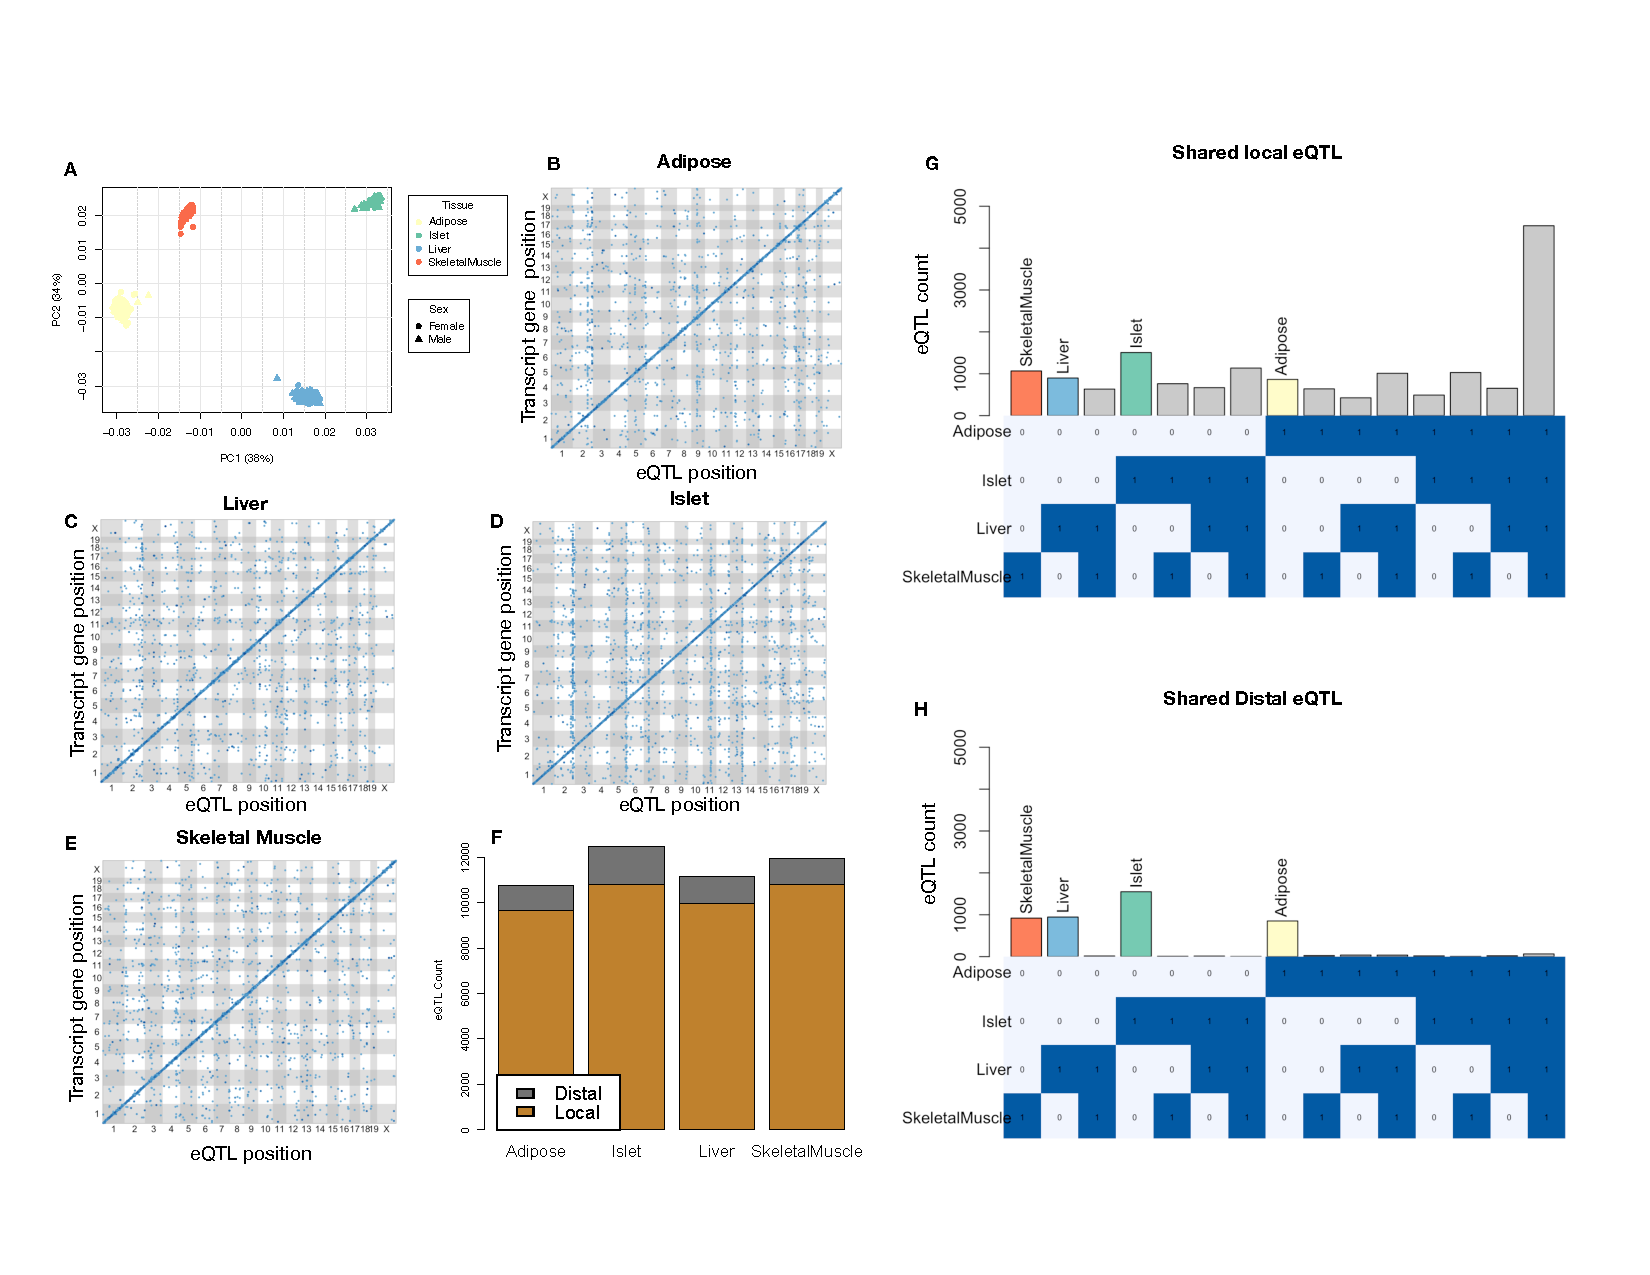
\includegraphics[width=\textwidth]{Figures/Supp_Fig1_eQTL.pdf} 
\caption{Overview of eQTL analysis in DO mice. \textbf{A.} RNA seq 
samples from the four different tissues clustered by tissue. 
\textbf{B.-E.} eQTL maps are shown for each tissue. The $x$-axis 
shows the position of the mapped eQTL, and the $y$-axis shows the 
physical position of the gene encoding each mapped transcript. 
Each dot represents an eQTL with a minimum LOD score of 8. The dots 
on the diagonal are locally regulated eQTL for which the mapped eQTL 
is at the within 4Mb of the encoding gene. Dots off the diagonal are 
distally regulated eQTL for which the mapped eQTL is distant from the 
gene encoding the transcript. \textbf{F.} Comparison of the total number 
of local and distal eQTL with a minimum LOD score of 8 in each tissue. 
All tissues have comparable numbers of eQTL. Local eQTL are much more 
numerous than distal eQTL. \textbf{G.} Counts of transcripts with local 
eQTL shared across multiple tissues. The majority of local eQTL were 
shared across all four tissues. \textbf{H.} Counts of transcripts with 
distal eQTL shared across multiple tissues. The majority of distal eQTL 
were tissue-specific and not shared across multiple tissues. For both G 
and H, eQTL for a given transcript were considered shared in two tissues 
if they were within 4Mb of each other. Colored bars indicate the counts 
for individual tissues for easy of visualization.
}
\label{fig:eQTL}
\end{figure}

\begin{figure}[ht!]
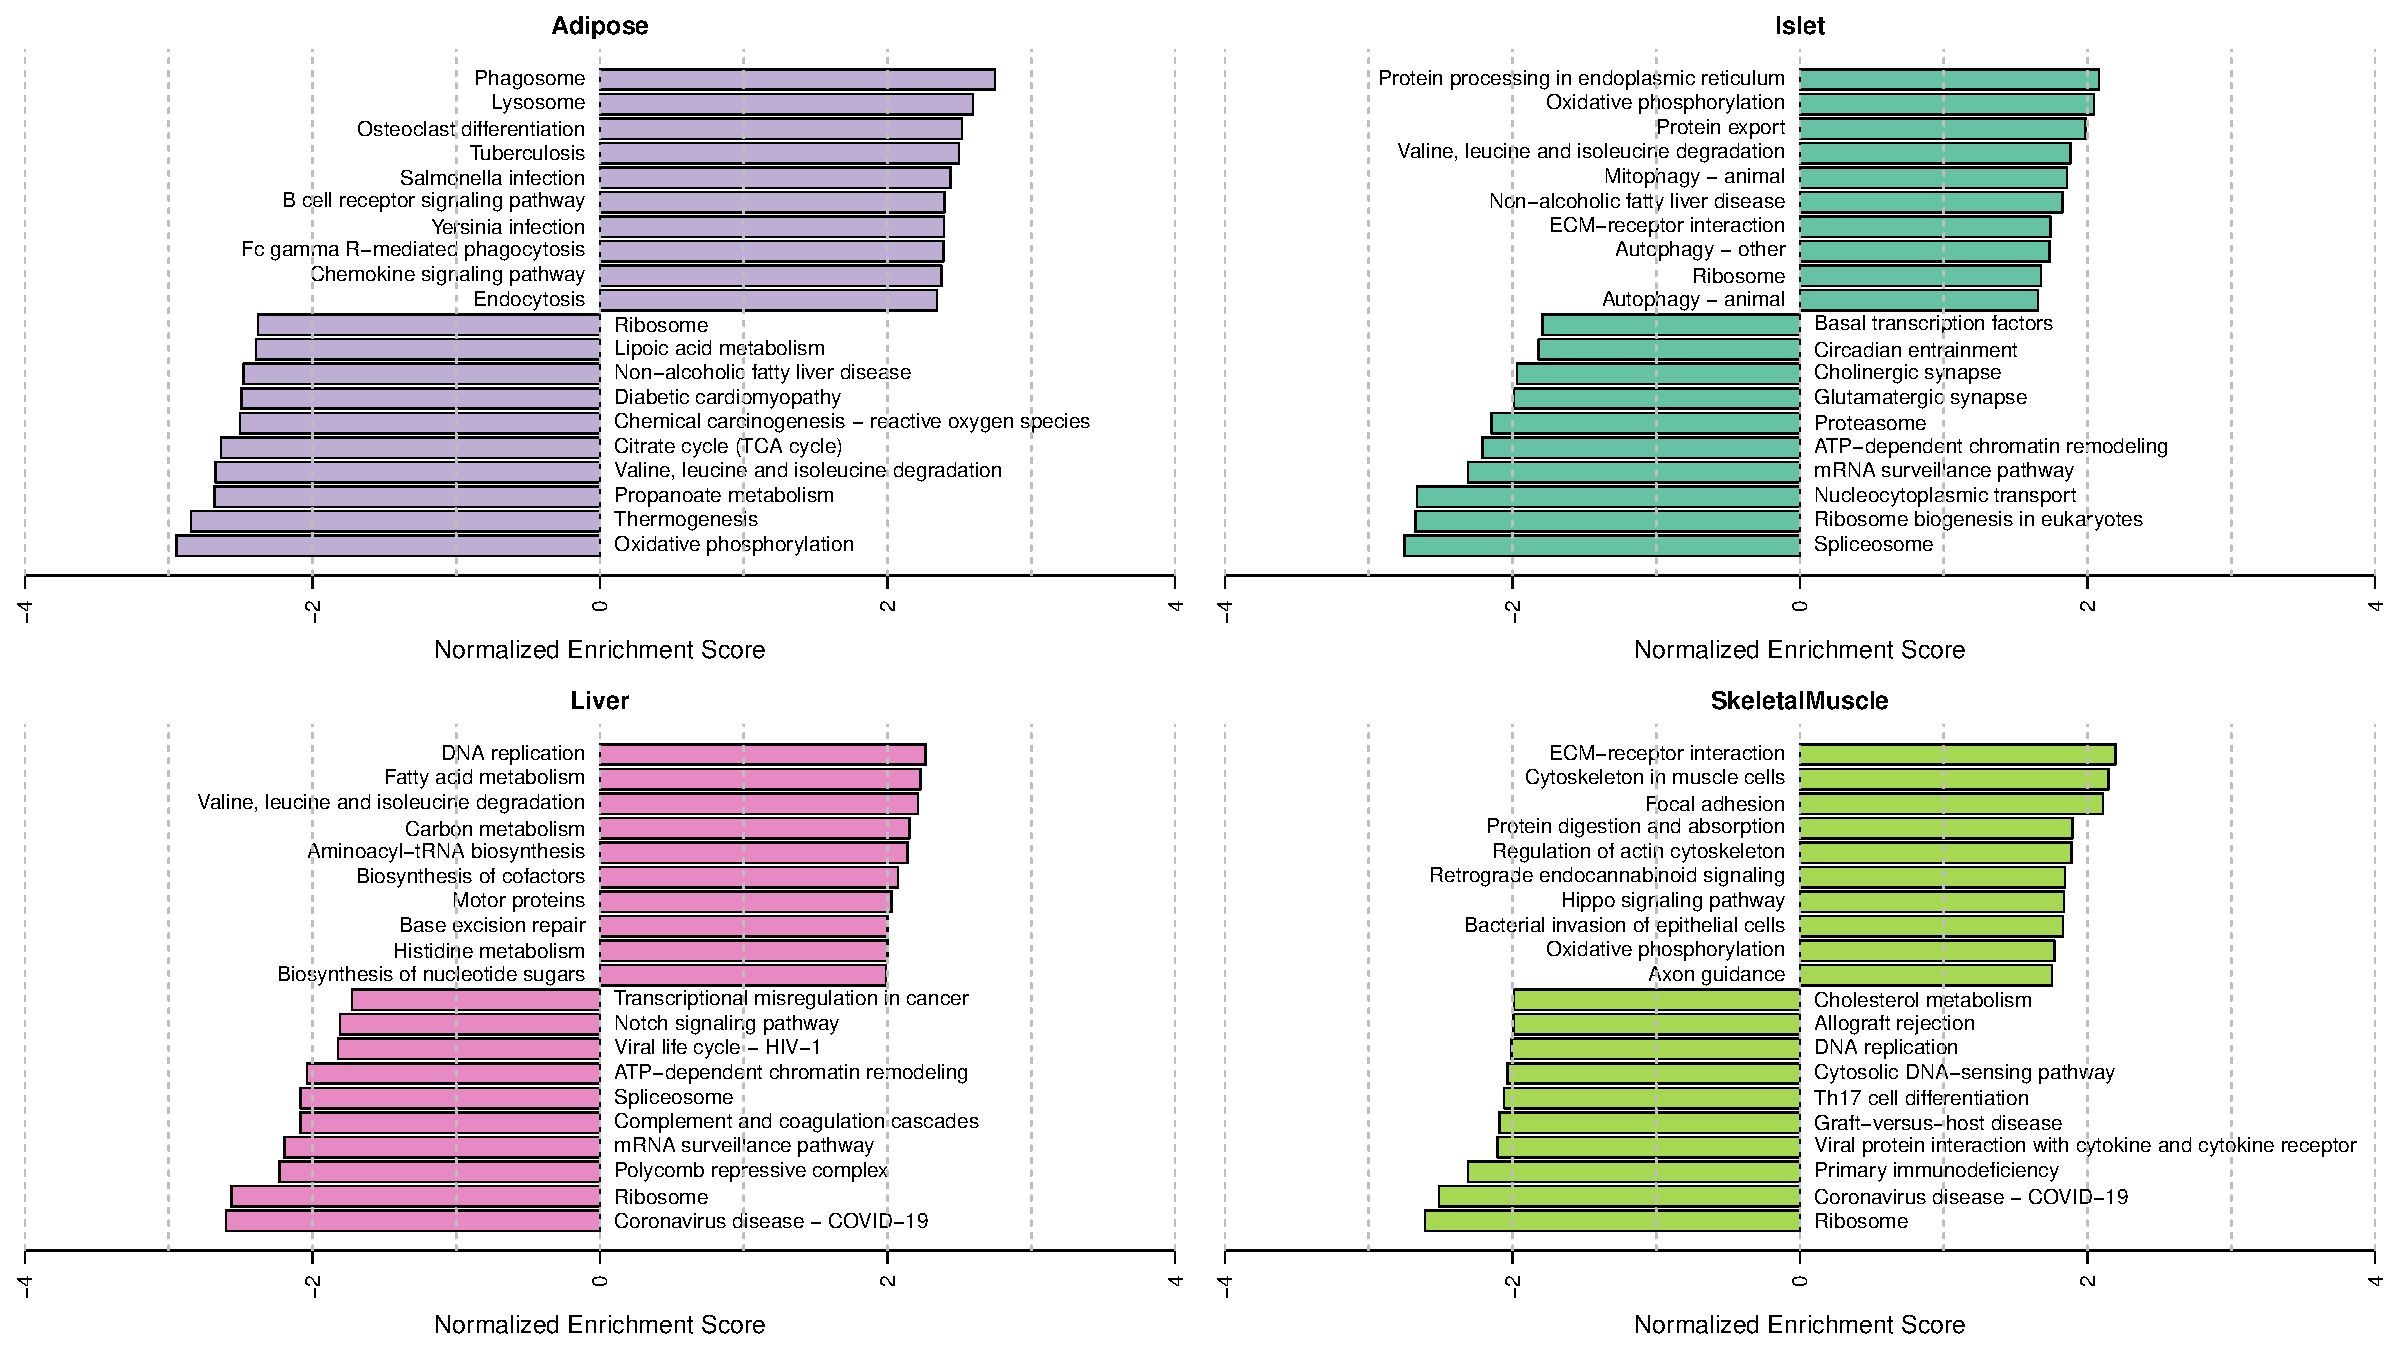
\includegraphics[width=\textwidth]{Figures/Supp_Fig_enrichments_KEGG.pdf} 
\caption{Bar plots showing normalized enrichment scores (NES) for KEGG 
pathways as determined by fast gene score enrichment analysis (fgsea). 
Only the top 10 positive and top 10 negative scores are shown. Colors 
indicate tissue. The name beside each bar shows the name of each enriched 
KEGG pathway.
}
\label{fig:top_enrich_kegg}
\end{figure}

\begin{figure}[ht!]
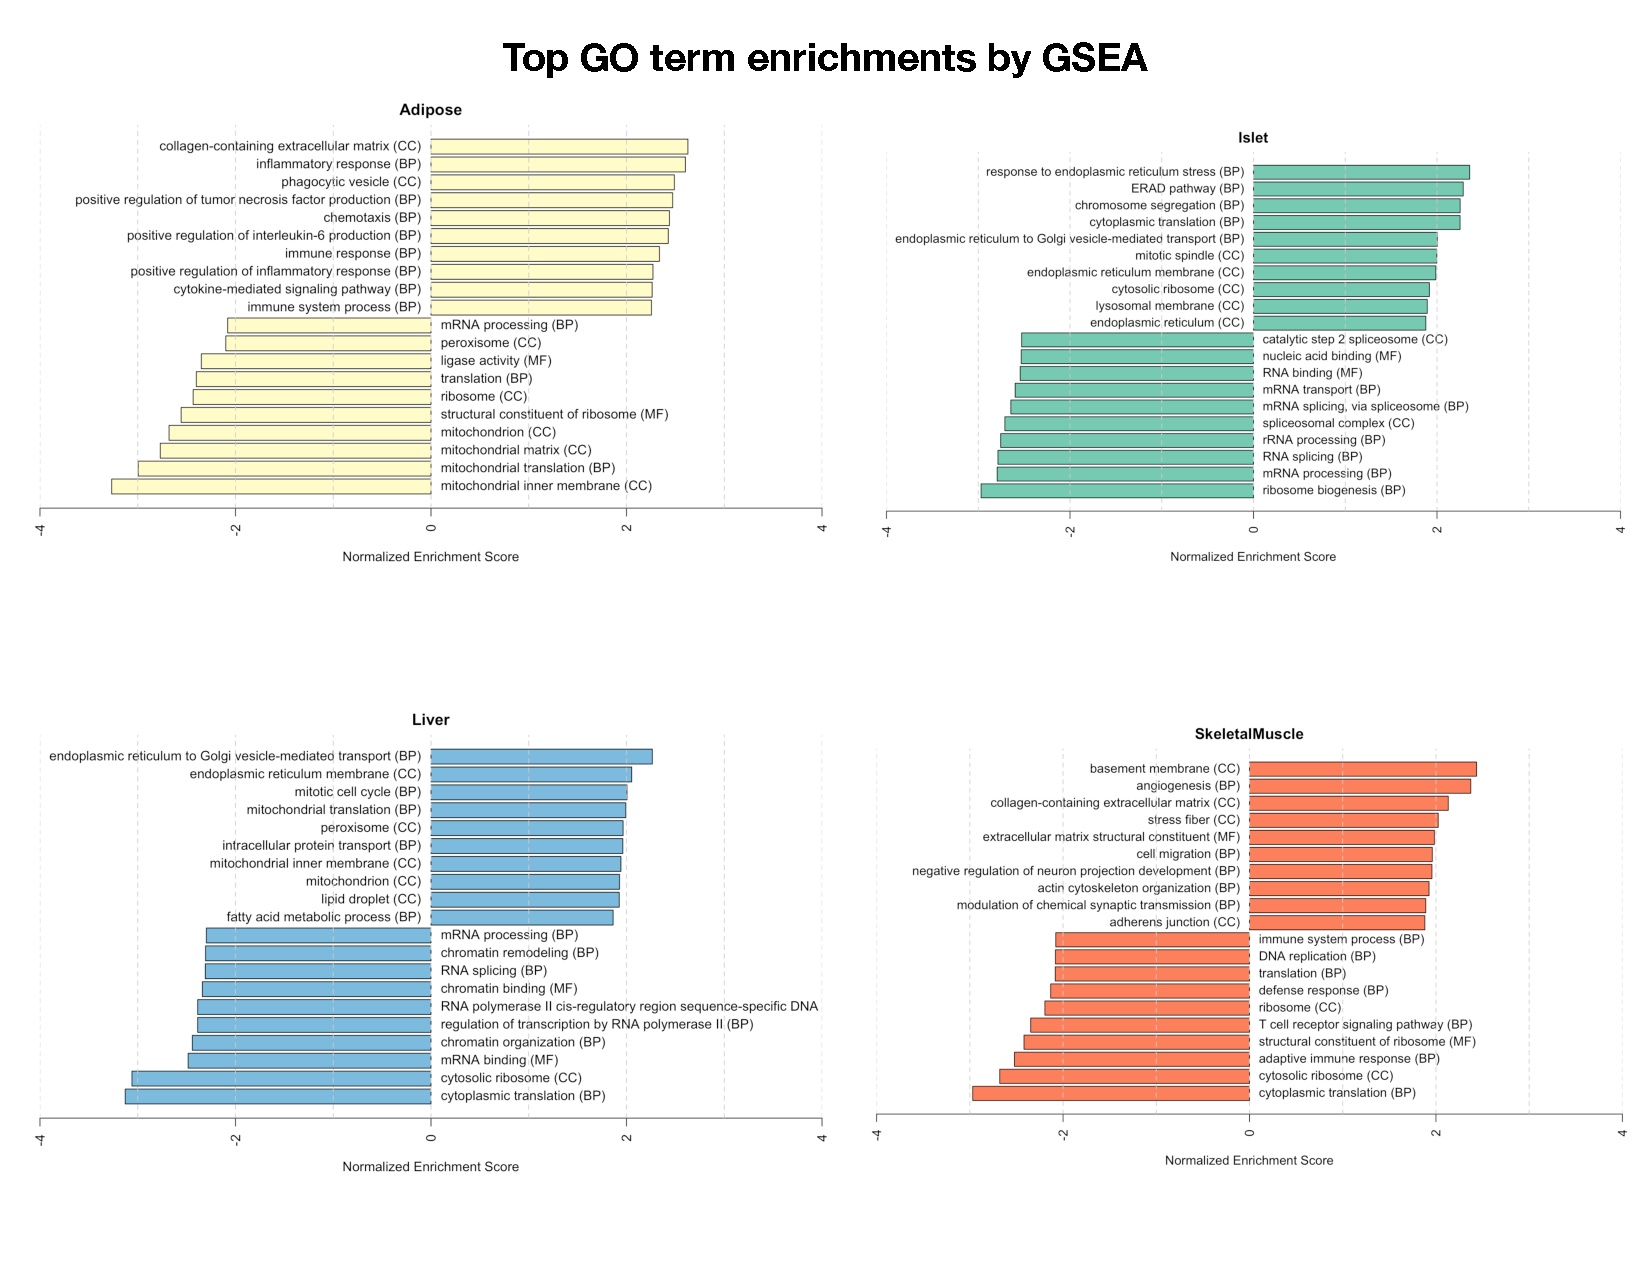
\includegraphics[width=\textwidth]{Figures/Supp_Fig_enrichments_GO.pdf} 
\caption{Bar plots showing normalized enrichment scores (NES) for GO 
terms as determined by fast gene score enrichment analysis (fgsea). 
Only the top 10 positive and top 10 negative scores are shown. Colors 
indicate tissue. The name beside each bar shows the name of each enriched 
GO term. The letters in parentheses indicate whether the term is from the 
biological process ontology (BP), the molecular function ontology (MF), 
or the cellular compartment ontology (CC).
}
\label{fig:top_enrich_go}
\end{figure}

\begin{figure}[ht!]
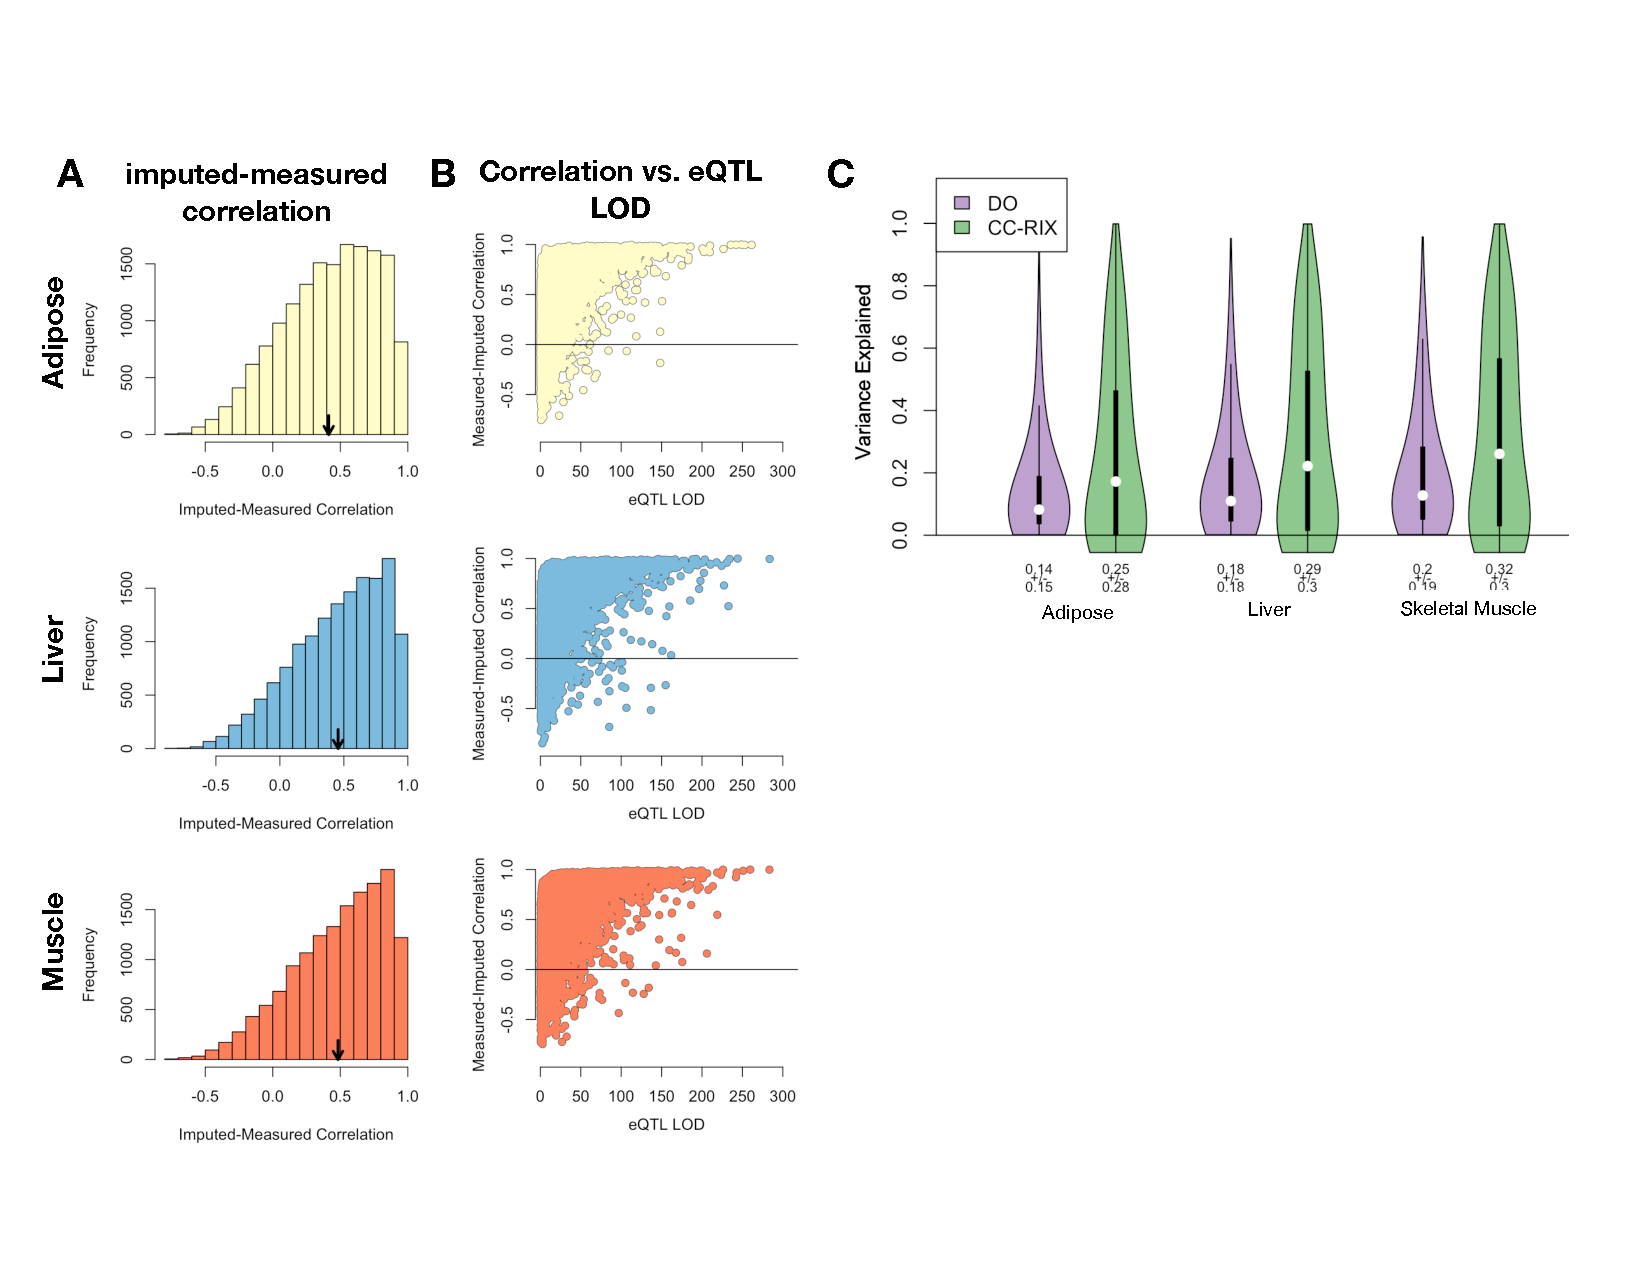
\includegraphics[width=\textwidth]{Figures/Supp_Fig_CC-RIX_Imputation.pdf} 
\caption{Validation of transcript imputation in the CC-RIX. \textbf{A.} 
Distributions of correlations between imputed and measured transcripts 
in the CC-RIX. The mean of each distribution is shown by the red line. 
All distributions were skewed toward positive correlations and had
 positive means near a Pearson correlation (r) of 0.5. \textbf{B.} 
 The relationship between the correlation between measured and 
 imputed expression in the CC-RIX (x-axis) and eQTL LOD score. As 
 expected, imputations are more accurate for transcripts with strong 
 local eQTL. \textbf{C.} Variance explained by local genotype in the 
 DO and CC-RIX. 
}
\label{fig:cc_imputation}
\end{figure}

\begin{figure}[ht!]
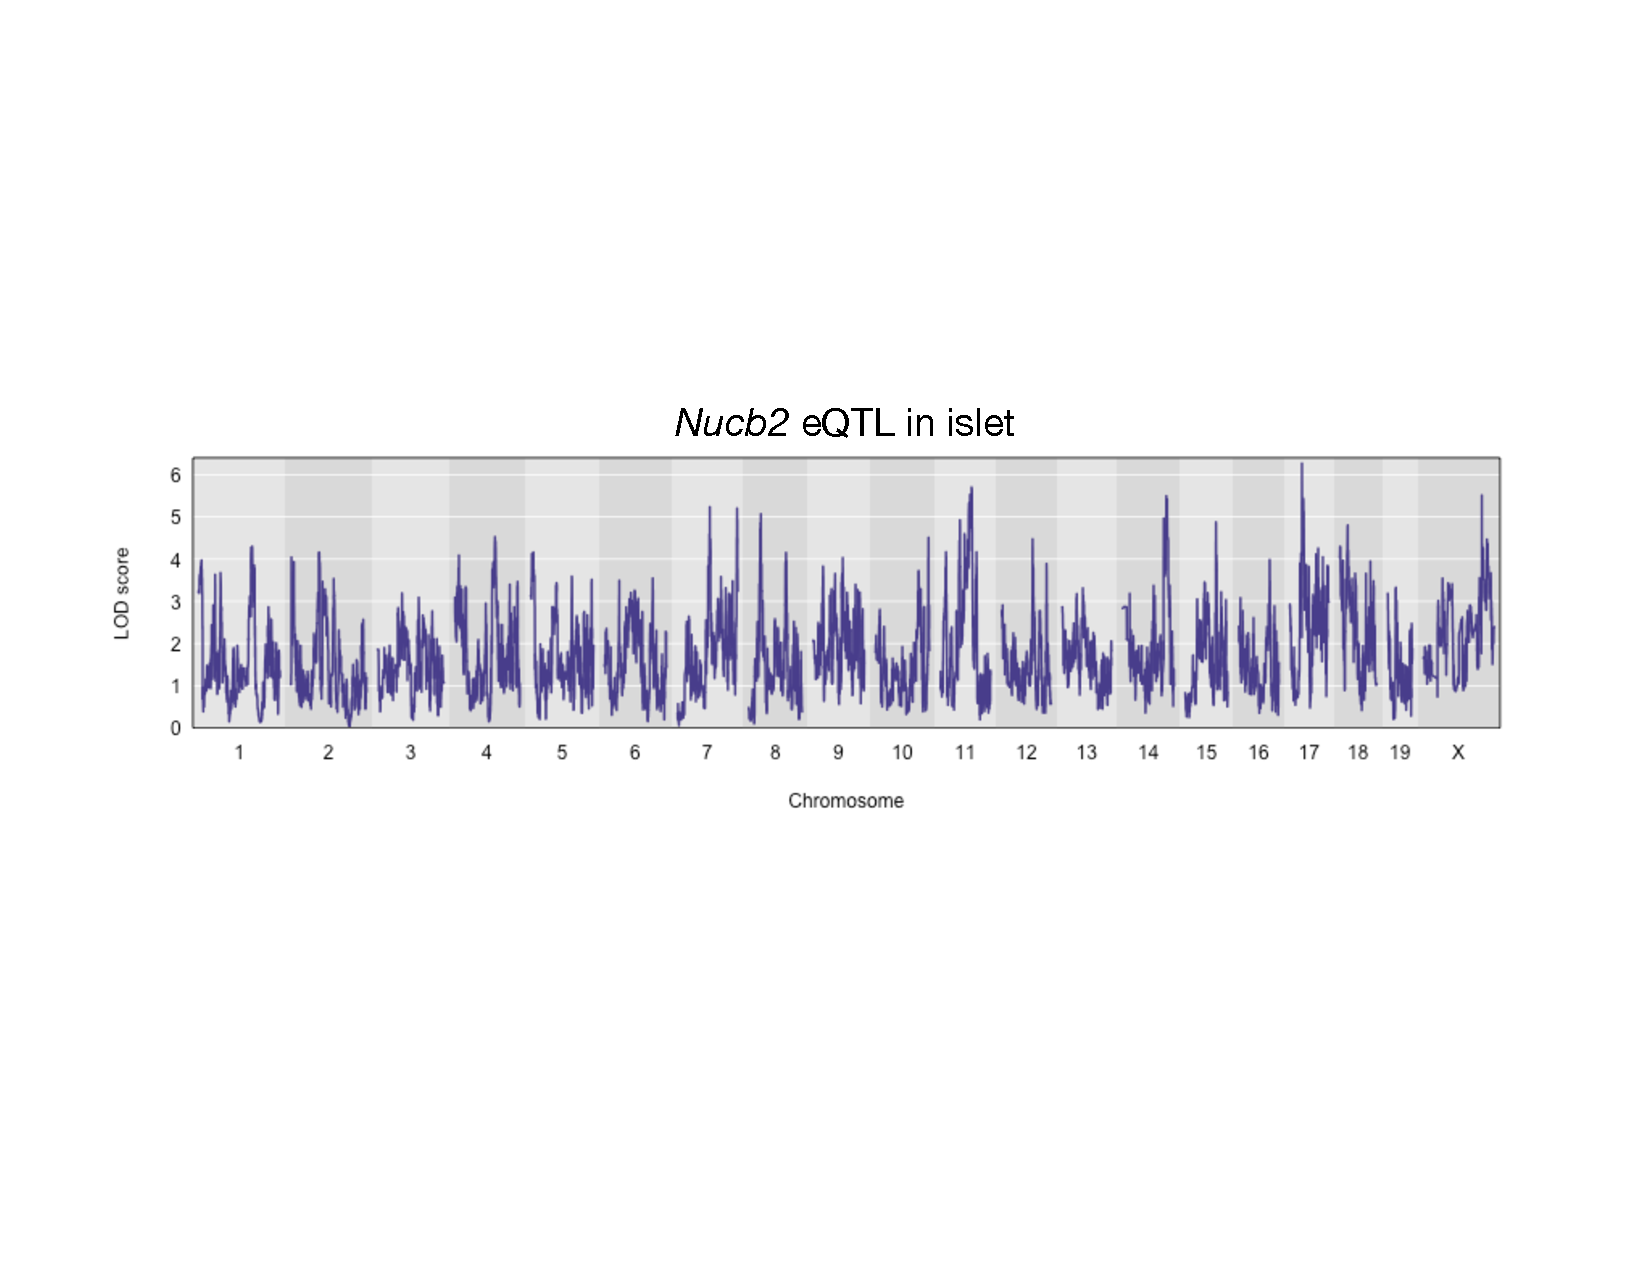
\includegraphics[width=\textwidth]{Figures/Supplemental_FigX_Nucb2_eQTL.pdf} 
\caption{Regulation of \textit{Nucb2} expression in islet. \textit{Nucb2} 
is encoded on mouse chromosome 7 at 116.5 Mb (red line). In islets the 
heritability of \textit{Nucb2} expression levels is 69\% heritable. This 
LOD score trace shows that there is no local eQTL at that position, nor 
any strong distal eQTL anywhere else in the genome. 
}
\label{fig:Nucb2_eqtl}
\end{figure}

\medskip

\bibliographystyle{unsrt}
\bibliography{islet.bib}

\end{document}
